% Options for packages loaded elsewhere
\PassOptionsToPackage{unicode}{hyperref}
\PassOptionsToPackage{hyphens}{url}
%
\documentclass[
]{article}
\usepackage{amsmath,amssymb}
\usepackage{lmodern}
\usepackage{iftex}
\ifPDFTeX
  \usepackage[T1]{fontenc}
  \usepackage[utf8]{inputenc}
  \usepackage{textcomp} % provide euro and other symbols
\else % if luatex or xetex
  \usepackage{unicode-math}
  \defaultfontfeatures{Scale=MatchLowercase}
  \defaultfontfeatures[\rmfamily]{Ligatures=TeX,Scale=1}
\fi
% Use upquote if available, for straight quotes in verbatim environments
\IfFileExists{upquote.sty}{\usepackage{upquote}}{}
\IfFileExists{microtype.sty}{% use microtype if available
  \usepackage[]{microtype}
  \UseMicrotypeSet[protrusion]{basicmath} % disable protrusion for tt fonts
}{}
\makeatletter
\@ifundefined{KOMAClassName}{% if non-KOMA class
  \IfFileExists{parskip.sty}{%
    \usepackage{parskip}
  }{% else
    \setlength{\parindent}{0pt}
    \setlength{\parskip}{6pt plus 2pt minus 1pt}}
}{% if KOMA class
  \KOMAoptions{parskip=half}}
\makeatother
\usepackage{xcolor}
\IfFileExists{xurl.sty}{\usepackage{xurl}}{} % add URL line breaks if available
\IfFileExists{bookmark.sty}{\usepackage{bookmark}}{\usepackage{hyperref}}
\hypersetup{
  hidelinks,
  pdfcreator={LaTeX via pandoc}}
\urlstyle{same} % disable monospaced font for URLs
\usepackage{color}
\usepackage{fancyvrb}
\newcommand{\VerbBar}{|}
\newcommand{\VERB}{\Verb[commandchars=\\\{\}]}
\DefineVerbatimEnvironment{Highlighting}{Verbatim}{commandchars=\\\{\}}
% Add ',fontsize=\small' for more characters per line
\newenvironment{Shaded}{}{}
\newcommand{\AlertTok}[1]{\textcolor[rgb]{1.00,0.00,0.00}{\textbf{#1}}}
\newcommand{\AnnotationTok}[1]{\textcolor[rgb]{0.38,0.63,0.69}{\textbf{\textit{#1}}}}
\newcommand{\AttributeTok}[1]{\textcolor[rgb]{0.49,0.56,0.16}{#1}}
\newcommand{\BaseNTok}[1]{\textcolor[rgb]{0.25,0.63,0.44}{#1}}
\newcommand{\BuiltInTok}[1]{#1}
\newcommand{\CharTok}[1]{\textcolor[rgb]{0.25,0.44,0.63}{#1}}
\newcommand{\CommentTok}[1]{\textcolor[rgb]{0.38,0.63,0.69}{\textit{#1}}}
\newcommand{\CommentVarTok}[1]{\textcolor[rgb]{0.38,0.63,0.69}{\textbf{\textit{#1}}}}
\newcommand{\ConstantTok}[1]{\textcolor[rgb]{0.53,0.00,0.00}{#1}}
\newcommand{\ControlFlowTok}[1]{\textcolor[rgb]{0.00,0.44,0.13}{\textbf{#1}}}
\newcommand{\DataTypeTok}[1]{\textcolor[rgb]{0.56,0.13,0.00}{#1}}
\newcommand{\DecValTok}[1]{\textcolor[rgb]{0.25,0.63,0.44}{#1}}
\newcommand{\DocumentationTok}[1]{\textcolor[rgb]{0.73,0.13,0.13}{\textit{#1}}}
\newcommand{\ErrorTok}[1]{\textcolor[rgb]{1.00,0.00,0.00}{\textbf{#1}}}
\newcommand{\ExtensionTok}[1]{#1}
\newcommand{\FloatTok}[1]{\textcolor[rgb]{0.25,0.63,0.44}{#1}}
\newcommand{\FunctionTok}[1]{\textcolor[rgb]{0.02,0.16,0.49}{#1}}
\newcommand{\ImportTok}[1]{#1}
\newcommand{\InformationTok}[1]{\textcolor[rgb]{0.38,0.63,0.69}{\textbf{\textit{#1}}}}
\newcommand{\KeywordTok}[1]{\textcolor[rgb]{0.00,0.44,0.13}{\textbf{#1}}}
\newcommand{\NormalTok}[1]{#1}
\newcommand{\OperatorTok}[1]{\textcolor[rgb]{0.40,0.40,0.40}{#1}}
\newcommand{\OtherTok}[1]{\textcolor[rgb]{0.00,0.44,0.13}{#1}}
\newcommand{\PreprocessorTok}[1]{\textcolor[rgb]{0.74,0.48,0.00}{#1}}
\newcommand{\RegionMarkerTok}[1]{#1}
\newcommand{\SpecialCharTok}[1]{\textcolor[rgb]{0.25,0.44,0.63}{#1}}
\newcommand{\SpecialStringTok}[1]{\textcolor[rgb]{0.73,0.40,0.53}{#1}}
\newcommand{\StringTok}[1]{\textcolor[rgb]{0.25,0.44,0.63}{#1}}
\newcommand{\VariableTok}[1]{\textcolor[rgb]{0.10,0.09,0.49}{#1}}
\newcommand{\VerbatimStringTok}[1]{\textcolor[rgb]{0.25,0.44,0.63}{#1}}
\newcommand{\WarningTok}[1]{\textcolor[rgb]{0.38,0.63,0.69}{\textbf{\textit{#1}}}}
\usepackage{graphicx}
\makeatletter
\def\maxwidth{\ifdim\Gin@nat@width>\linewidth\linewidth\else\Gin@nat@width\fi}
\def\maxheight{\ifdim\Gin@nat@height>\textheight\textheight\else\Gin@nat@height\fi}
\makeatother
% Scale images if necessary, so that they will not overflow the page
% margins by default, and it is still possible to overwrite the defaults
% using explicit options in \includegraphics[width, height, ...]{}
\setkeys{Gin}{width=\maxwidth,height=\maxheight,keepaspectratio}
% Set default figure placement to htbp
\makeatletter
\def\fps@figure{htbp}
\makeatother
\setlength{\emergencystretch}{3em} % prevent overfull lines
\providecommand{\tightlist}{%
  \setlength{\itemsep}{0pt}\setlength{\parskip}{0pt}}
\setcounter{secnumdepth}{-\maxdimen} % remove section numbering
\ifLuaTeX
  \usepackage{selnolig}  % disable illegal ligatures
\fi

\author{}
\date{}

\begin{document}

\hypertarget{proyecto-de-anuxe1lisis-de-datos}{%
\section{Proyecto de Análisis de
Datos}\label{proyecto-de-anuxe1lisis-de-datos}}

En este trabajo analizamos los datos abiertos del programa de
\href{https://mibici.net}{renta de bicicletas} "Mi Bici" de la zona
metropolitana de Guadalajara. En particular nos interesa conocer el
impacto que han tenido políticas de ampliación del programa y las
políticas de distanciamiento social derivadas de la pandemia. Con este
análisis esperamos brindar información que permita evaluar el programa
de renta de bicicletas.

Para hacer este análisis, el presente reporte se divide de la siguiente
forma:

\begin{itemize}
\item
  En la sección
  \protect\hyperlink{anuxe1lisis-exploratorio-de-datos}{Análisis
  Exploratorio de Datos} describimos brevemente la información que
  incluye los datos y algunos descubrimientos que hicimos explorando y
  graficando algunas variables
\item
  En la sección \protect\hyperlink{cambios-de-estructura}{Cambios de
  Estructura} explicamos cómo es posible obtener puntos de quiebre donde
  la estructura de la serie de tiempo cambia, además interpretamos los
  resultados obtenidos al usar dichos métodos
\item
  En la sección
  \protect\hyperlink{anuxe1lisis-de-las-estaciones}{Análisis de las
  estaciones} tratamos de proporcionar gráficas informativas sobre el
  uso de las estaciones en las diferentes etapas del programa
\item
  Finalmente, en
  \protect\hyperlink{conclusiones-y-comentarios-finales}{Conclusiones y
  Comentarios Finales} damos algunas conclusiones y trabajo a
  desarrollar en el futuro
\end{itemize}

Sin más preámbulo, pasamos a describir la limpieza de los datos y los
resultados de su análisis exploratorio.

\begin{center}\rule{0.5\linewidth}{0.5pt}\end{center}

\hypertarget{anuxe1lisis-exploratorio-de-datos}{%
\subsection{Análisis Exploratorio de
Datos}\label{anuxe1lisis-exploratorio-de-datos}}

Los datos proporcionados por Mi Bici están disposibles en agregados
mensuales. Cada archivo consiste en una tabla que proporciona para cada
viaje:

\begin{itemize}
\item
  Un Identificador único del viaje
\item
  El identificador del usuario que realiza el viaje
\item
  Género del usuario
\item
  Año de nacimiento del usuario
\item
  Fecha y hora del inicio del viaje
\item
  Fecha y hora del fin del viaje
\item
  Identificador de la estación de origen
\item
  Indentificación de la estación destino
\end{itemize}

Como para responder nuestras preguntas, solo necesitamos el número de
viajes por intervalo de tiempo, decidimos contar el número de viajes
realizados al día. El resultado fue el siguiente:

\begin{figure}
\centering
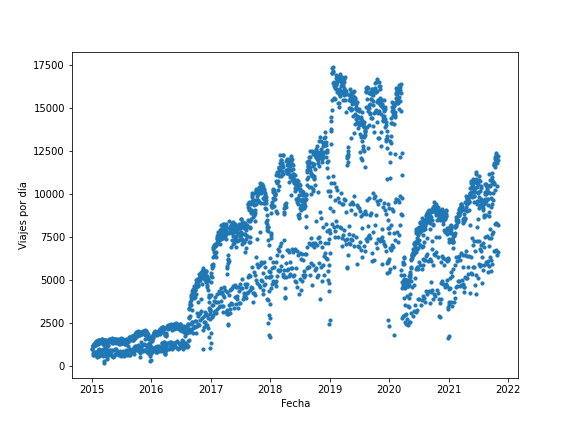
\includegraphics{/Users/jaimefco/Documents/AnalisisDeDatos/proyecto/plots/trips_daily.png}
\caption{}
\end{figure}

En esta gráfica se observa el número de viajes por día, desde el enero
de 2015 hasta octubre de 2021.

En la gráfica se aprecia como hay una gran variabilidad de un día a
otro. De hecho, podemos encontrar al menos dos grupos diferenciados, uno
arriba y otro abajo. Para distiguir los días de mejor manera, agrupamos
por días de la semana obtieniendo lo siguiente:

\begin{figure}
\centering
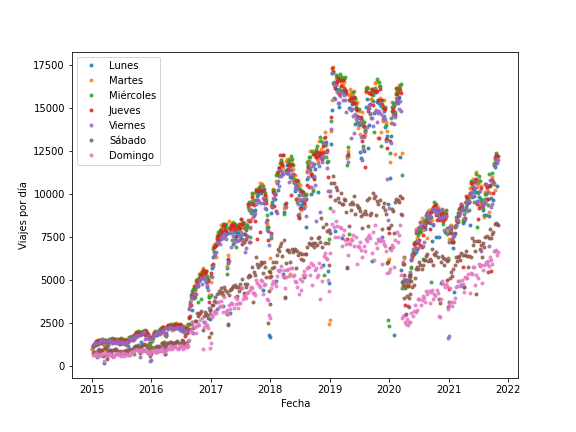
\includegraphics{/Users/jaimefco/Documents/AnalisisDeDatos/proyecto/plots/trips_daily_by_day.png}
\caption{}
\end{figure}

Podemos observar como sábados y domingos tenemos una baja en el número
de viajes. Más evidente es en la siguiente gráfica.

\begin{figure}
\centering
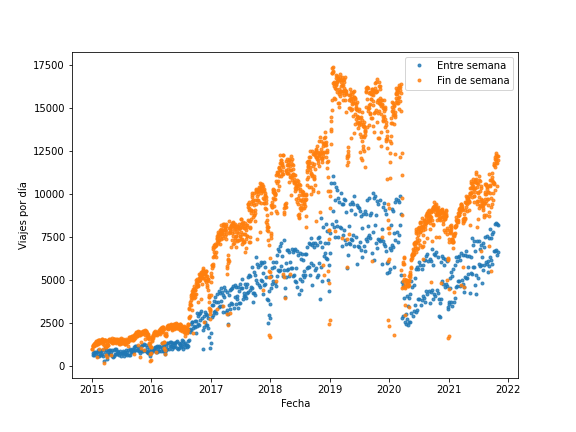
\includegraphics{/Users/jaimefco/Documents/AnalisisDeDatos/proyecto/plots/trips_daily_by_weekend.png}
\caption{}
\end{figure}

Puesto que no queremos que nuestros métodos para evaluar el cambio de
estructura se vean afectados por el cambio en los días de la semana,
decidimos agregar el número de viajes realizados cada semana (empezando
en lunes). El número de viajes por se mana presenta la siguiente
estructura:

\begin{figure}
\centering
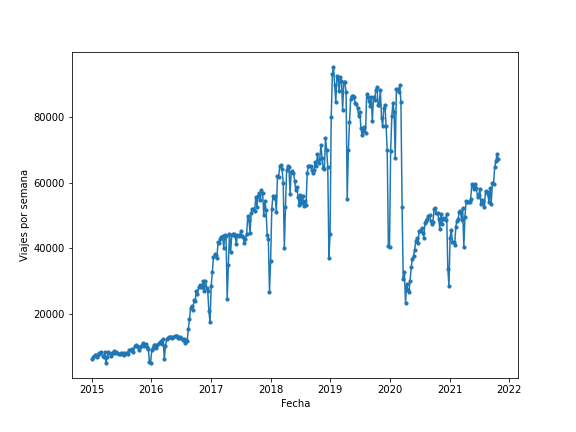
\includegraphics{/Users/jaimefco/Documents/AnalisisDeDatos/proyecto/plots/trips_weekly.png}
\caption{}
\end{figure}

Se observa una serie de tiempo más uniforme con pequeñas caidas en lo
que suponemos son semanas con fines de semana largos o vacaciones. De ya
se puede apreciar una caida en el númeri de viajes a inicio del 2020,
seguramente provocada por las medidas de confinamiento implementadas en
la entidad al inicio de la pandemia.

También nos interesó contabilizar el número de viajes realizados entre
pares de estaciones, el prrocesamiento de esos datos se detalla en la
penúltima sección.

\begin{center}\rule{0.5\linewidth}{0.5pt}\end{center}

\hypertarget{cambios-de-estructura}{%
\subsection{Cambios de estructura}\label{cambios-de-estructura}}

\begin{figure}
\centering
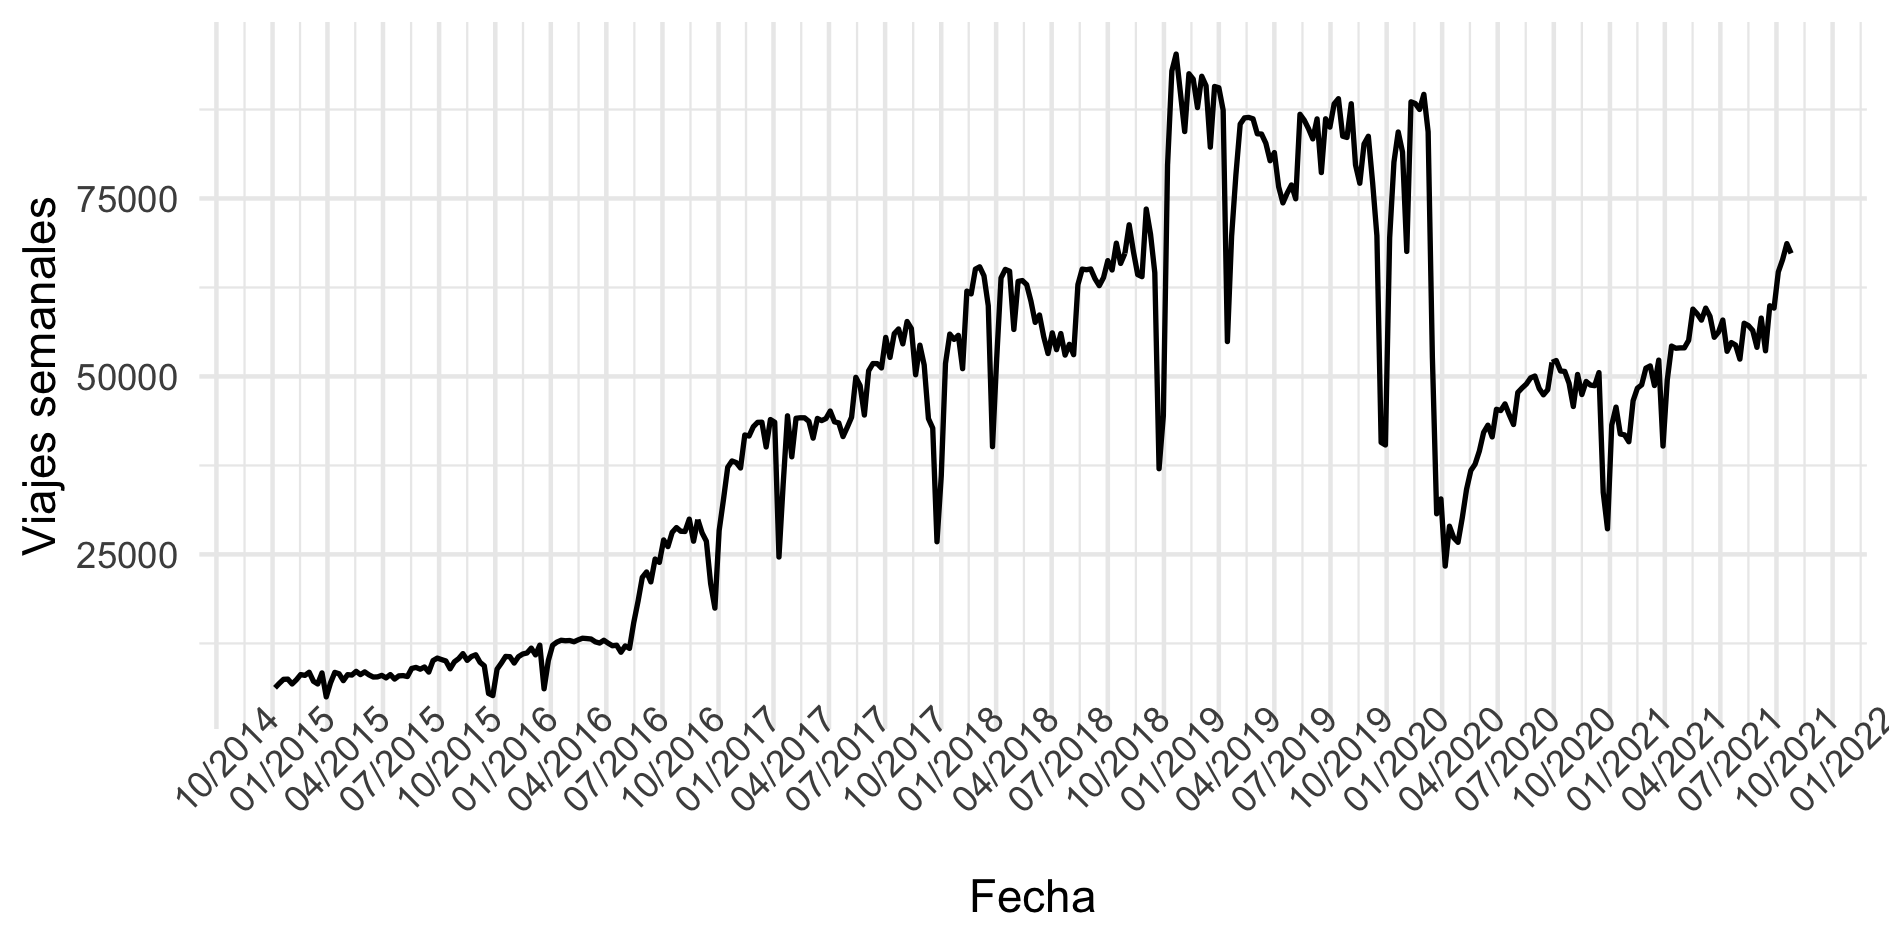
\includegraphics{/Users/jaimefco/Documents/AnalisisDeDatos/proyecto/plots/serie1.png}
\caption{}
\end{figure}

Dado un conjunto de datos \(\{(Y_i, X_i)\}_{i=1}^n\) con \(X_i \in \mathbb{R}\),
suponemos que existen \(k\) intervalos \([a_i, a_{i+1}]\) para
\(i \in \{1, \dots, k\}\), de forma tal que es posible dividir las
observaciones en estos intervalos, es decir para índices en \(I_j\) ,
\((Y_i, X_i)_{i \in I_j} \in [a_j, a_j+1]\) de forma tal que hay una
relación lineal entre estos datos que puede o no estar relacionada con
el modelo lineal de los otros intervalos.

¿Bajo qué condiciones se puede dar este supuesto? Es posible que se
tenga un experimento a través del tiempo donde las condiciones las
experimento cambian por una cierta temporalidad. En nuestro caso
queremos probar la hipótesis de que el comportamiento del número de
viajes realizados ha cambiado por la pandemia o no.

De ser cierta la hipótesis, se dice que los datos presentan un
\textbf{cambio de estructura} y a los puntos \(a_2, \dots, a_{k-1}\)
como \textbf{punto de quiebre}. El problema cambia dependiendo de la
información que poseemos.

Estudiemos primero el caso donde conocemos que existe un solo punto de
quiebre y nos interesa evaluar la hipótesis

\(H_0: \text{no existe cambio de estructura.}\)

La hipótesis puede ser descrita formalmente de la siguiente forma:

\(H_0: Y_i = \beta X_i + u_i, \quad \forall i\in\{1, \dots, n\},\)

mientras que la hipótesis alternativa sería:
\begin{equation*}
   H_1: \exists \quad i_0 \in \{1, \dots, n\} \text{ tal que }
   \begin{cases}
      Y_i = \beta_A X_i + u_i \quad 1 \leq i \leq i_0\\
      Y_i = \beta_B X_i + u_i \quad i_0 < i \leq n
   \end{cases},\beta_A \neq \beta_B.
\end{equation*}

\href{https://www.jstor.org/stable/1910133}{Chow (1960)} propuso un
estadísitico que puede ser usado para probar esta hipótesis cuando el
valor \(i_0\) es conocido. Para ello propone ajustar dos modelos de
regresión lineal de forma independiente para cada uno de los dos
intervalos definidos por \(i_0\), y rechazar la hipótesis alternativa si
el cociente:

\[F_{i_0} = \frac{\hat u^\top \hat u - \hat e ^\top \hat e}{\hat e^\top \hat e / (n - 2)}\]

es mayor que un cierto valor, donde
\(\hat e = (\hat u_A, \hat u_B)\top\) son los residuales de cada modelo
de regresión ajustado de forrma independiente en su intervalo y
\(\hat u\) son los residuales del modelo lineal ajustado a toda la
muestra.

Chow demuestra que bajo \(H_0\), el estadísitico se distribuye
asintóticamente una \(\chi^2_1\) y, si \(u_i \sim \mathcal N\), el
estadísitico \(F_{i_0}\) sigue una distribución \(F\) con \(n-2\) grados
de libertad.

Sin embargo, dado que desconocemos el valor de \(i_0\),
\href{https://www.jstor.org/stable/2951764}{Andrews (1993)} propone
calcular el estadístico \(F\) para todos los posibles puntos de quiebre
y rechazar la hipótesis nula si para alguno se llega a un valor alto.
Para deterrminar si alguno de los valores llega a ser alto, se puede
usar el estadístico:

\(\sup F = \sup_{1< i <n} F_i.\)

Usando este estadístico de prueba, evaluamos la hipótesis nula para
saber si existe evidencia suficiente para suponer que la pandemia ha
provocado un cambio en la estructura del número de viajes que se
realizan en el sitema MiBici de Guadalajara.

\hypertarget{experimentos-con-un-solo-punto-de-quiebre}{%
\subsubsection{Experimentos con un solo punto de
quiebre}\label{experimentos-con-un-solo-punto-de-quiebre}}

Usando la librería \texttt{strucchange} de \texttt{R}, calculamos
estadístico \(F\) para todo punto en nuestros datos. Esto se puede
realizar con la función \texttt{Fstats}. Observe que para los modelos de
regresión usamos como único predictor el tiempo.

\begin{Shaded}
\begin{Highlighting}[]
\NormalTok{res }\OtherTok{\textless{}{-}} \FunctionTok{Fstats}\NormalTok{(trips }\SpecialCharTok{\textasciitilde{}}\NormalTok{ date }\SpecialCharTok{+} \DecValTok{1}\NormalTok{, }\AttributeTok{data =}\NormalTok{ data) }\CommentTok{\# F statistics}

\FunctionTok{plot}\NormalTok{(res2, }\AttributeTok{xaxt =} \StringTok{"n"}\NormalTok{, }\AttributeTok{xlab =} \StringTok{""}\NormalTok{) }\CommentTok{\# Plot F statistics}
\FunctionTok{axis}\NormalTok{(}\DecValTok{1}\NormalTok{, }\AttributeTok{labels=}\NormalTok{labels, }\AttributeTok{at =}\NormalTok{ ticks}\SpecialCharTok{/}\FunctionTok{length}\NormalTok{(data}\SpecialCharTok{$}\NormalTok{X), }\AttributeTok{las=}\DecValTok{2}\NormalTok{)}
\CommentTok{\# Print line at i arg sup F}
\FunctionTok{breakpoints}\NormalTok{(res2)}
\FunctionTok{lines}\NormalTok{(}\FunctionTok{breakpoints}\NormalTok{(res2))}
\end{Highlighting}
\end{Shaded}

En los resultados observmos un linea punteada el posible punto de
quiebre para el cual se obtiene el valor del estadísitico \(F\) más
alto.

\begin{verbatim}
	 Optimal 2-segment partition:

Call:
breakpoints.Fstats(obj = res2)
\end{verbatim}

\begin{figure}
\centering

\includegraphics{/Users/jaimefco/Documents/AnalisisDeDatos/proyecto/plots/structChange_files/structChange_9_1.png}
\caption{}
\end{figure}

Note que el máximo lo obtenemos en fechas cercanas a febrero de 2020.
Además observamos como todos los valores rebasan la linea roja que
corresponde al valor máximo de la prueba a nivel \(\alpha=0.05\). Quiere
decir que con un nivel del 95 \%, rechazamos la hipótesis nula para
cualquier punto.

El p-valor sorrespondiente a \(\sup F\) es menor a \(10^{-15}\).
Practicamente 0.

\begin{Shaded}
\begin{Highlighting}[]
\FunctionTok{sctest}\NormalTok{(res, }\AttributeTok{type=}\StringTok{"supF"}\NormalTok{)}
\end{Highlighting}
\end{Shaded}

\begin{verbatim}
	supF test

data:  res2
sup.F = 1358.7, p-value < 2.2e-16
\end{verbatim}

Podemos graficar los modelos de regresión que resultan para cada
intervalo. Estos se ven así:\\
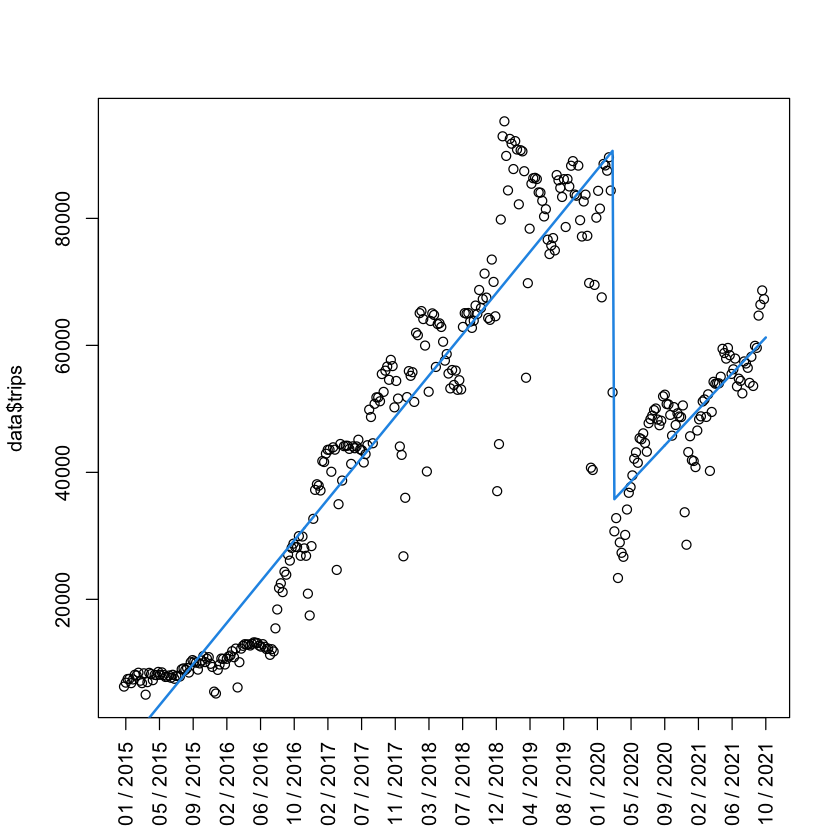
\includegraphics{/Users/jaimefco/Documents/AnalisisDeDatos/proyecto/plots/structChange_files/structChange_15_0.png}

Se aprecia como ambas rectas aproximan bien los datos. Sin embargo
observamos que existe un comportamiento diferente en 2015 y 2016,
comparrado con 2017 a 2019. Esto puede ser un indicativo de más cambios
de estructura que los que contemplamos originalmente.

Antes de evaluar esta posibilidad, vamos a ubicar con precisión el punto
de quiebre obtenido y evaluar la calidad de los modelos lineales
ajustados.

\begin{Shaded}
\begin{Highlighting}[]
\NormalTok{bp }\OtherTok{\textless{}{-}} \FunctionTok{breakpoints}\NormalTok{(res)}
\end{Highlighting}
\end{Shaded}

\begin{Shaded}
\begin{Highlighting}[]
\NormalTok{data}\SpecialCharTok{$}\NormalTok{date[bp}\SpecialCharTok{$}\NormalTok{breakpoint]}
\end{Highlighting}
\end{Shaded}

2020-03-09

Se observa que el punto de quiebre obtenido corresponde a la semana del
9 de marzo de 2020, que corresponde con la semana de
\href{https://www.animalpolitico.com/2020/03/jalisco-suspende-clases-universidades-eventos-masivos-coronavirus/}{suspensión
de clases presenciales} es el estado de Jalisco.

Por otro lado, los modelos de regresión parecen ajustarse bien a los
datos:

\begin{Shaded}
\begin{Highlighting}[]
\NormalTok{fm1 }\OtherTok{\textless{}{-}} \FunctionTok{lm}\NormalTok{(trips }\SpecialCharTok{\textasciitilde{}} \FunctionTok{breakfactor}\NormalTok{(bp)}\SpecialCharTok{/}\NormalTok{date }\SpecialCharTok{{-}} \DecValTok{1}\NormalTok{, }\AttributeTok{data =}\NormalTok{ data)}
\end{Highlighting}
\end{Shaded}

\begin{Shaded}
\begin{Highlighting}[]
\FunctionTok{summary}\NormalTok{(fm1)}
\end{Highlighting}
\end{Shaded}

\begin{verbatim}
Call:
lm(formula = trips ~ breakfactor(bp)/date - 1, data = data)

Residuals:
   Min     1Q Median     3Q    Max
-46783  -4269    467   5072  25152

Coefficients:
                               Estimate Std. Error t value Pr(>|t|)
breakfactor(bp)segment1      -8.191e+05  1.614e+04 -50.743  < 2e-16 ***
breakfactor(bp)segment2      -7.583e+05  9.845e+04  -7.702 1.37e-13 ***
breakfactor(bp)segment1:date  4.963e+01  9.281e-01  53.478  < 2e-16 ***
breakfactor(bp)segment2:date  4.330e+01  5.284e+00   8.195 4.70e-15 ***
---
Signif. codes:  0 ‘***’ 0.001 ‘**’ 0.01 ‘*’ 0.05 ‘.’ 0.1 ‘ ’ 1

Residual standard error: 8367 on 352 degrees of freedom
Multiple R-squared:  0.974,	Adjusted R-squared:  0.9737
F-statistic:  3297 on 4 and 352 DF,  p-value: < 2.2e-16
\end{verbatim}

Los p-valores del estadístico \(T\) son muy chicos y
\(R^2 \approx 0.97\), muy cerca de \(1\).

\hypertarget{experimentos-con-muxfaltiples-puntos-de-quiebre}{%
\subsubsection{Experimentos con múltiples puntos de
quiebre}\label{experimentos-con-muxfaltiples-puntos-de-quiebre}}

Dado que para muchos valores obtenemos un valor alto de \(F\) y por la
inspección visual de los datos, es razonable pensar en la existencia de
más puntos de quiebre en nuestros datos. Para ello podemos usar el mismo
razonamiento hecho con anterioridad, pero ahora evaluar el estadísitico
para los dos intervalos obtenidos. Esto es, hacer un análisis para el
intervalo que va del primero de enero de 2015 al 9 de marzo de 2020, y
otro para el intervalo del 9 de marzo de 2020 a la fecha.

Sin embargo este enfoque solo nos va a permitir determinar un punto de
quiebre a la vez. Los autores de la librería \texttt{strucchange} ponen
a nuestra disposición algunos métodos más elaborados para la detección
de multiples puntos de quiebre. Dentro de sus propuestas se considera un
proceso de fluctuación basado en estimar de forma recursiva modelos de
regresión lineal para diferentes ventanas de tiempo. Dado que el estudio
de estos procesos de fluctuación están fuera del alcance del curso, nos
limitamos a utilizar dicha función y discutir los modelos de regresión
que se ajustan con los nuevos puntos de quiebre.

La función
\texttt{efp(trips\ \textasciitilde{}\ date\ +\ 1,\ data\ =\ data,\ type\ =\ "ME")}
realiza el análisis y regresa los posibles puntos de quiebre. Lo que es
de nuestro interés, es analizar el \emph{residual sum of squares} cuando
ajustamos un solo modelo de regrresión lineal, dos modelos, tres modelos
o cuatro modelos dependiendo del número de quiebres que obtenemos. Esto
se puede apreciar en la siguiente gráfica:

\begin{figure}
\centering
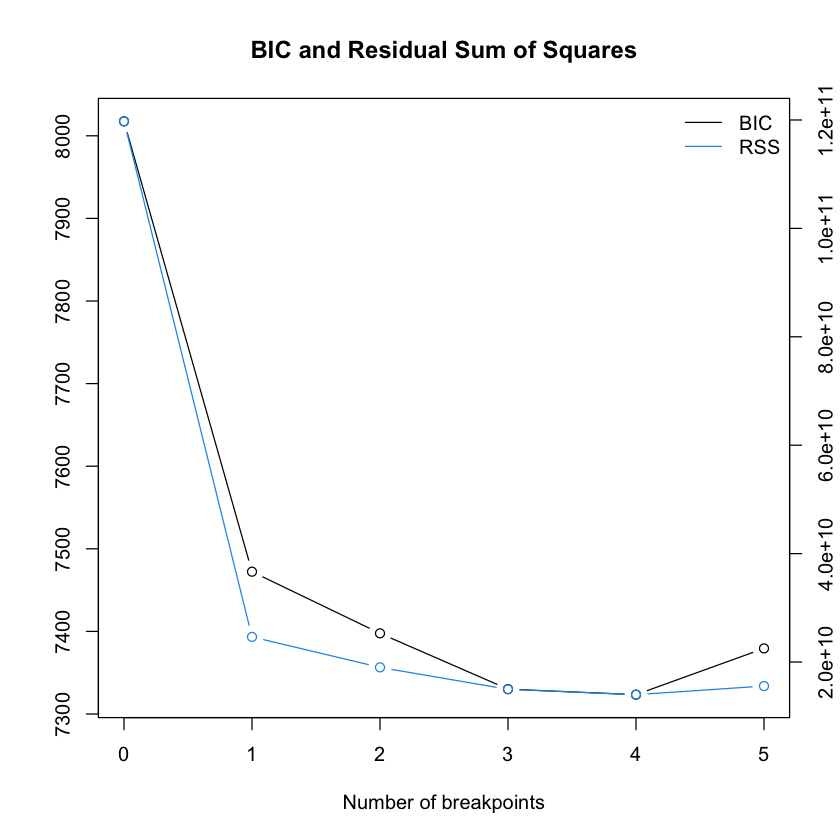
\includegraphics{/Users/jaimefco/Documents/AnalisisDeDatos/proyecto/plots/structChange_files/structChange_17_3.png}
\caption{}
\end{figure}

Podemos destacar que el cambio en el error disminuye considerablemente
de 0 a 1 punto de quiebre. Este punto corresponde al ya analizado. Por
otro lado, se observa que después del cuarto punto de quiebre, el error
aumenta. Después de una inspección visual de los modelos de regresión,
decidimos quedarnos con los primeros tres puntos de quiebre, pues se
ajustan muy bien a los datos como se muestra en la siguiente imagen:

\begin{figure}
\centering
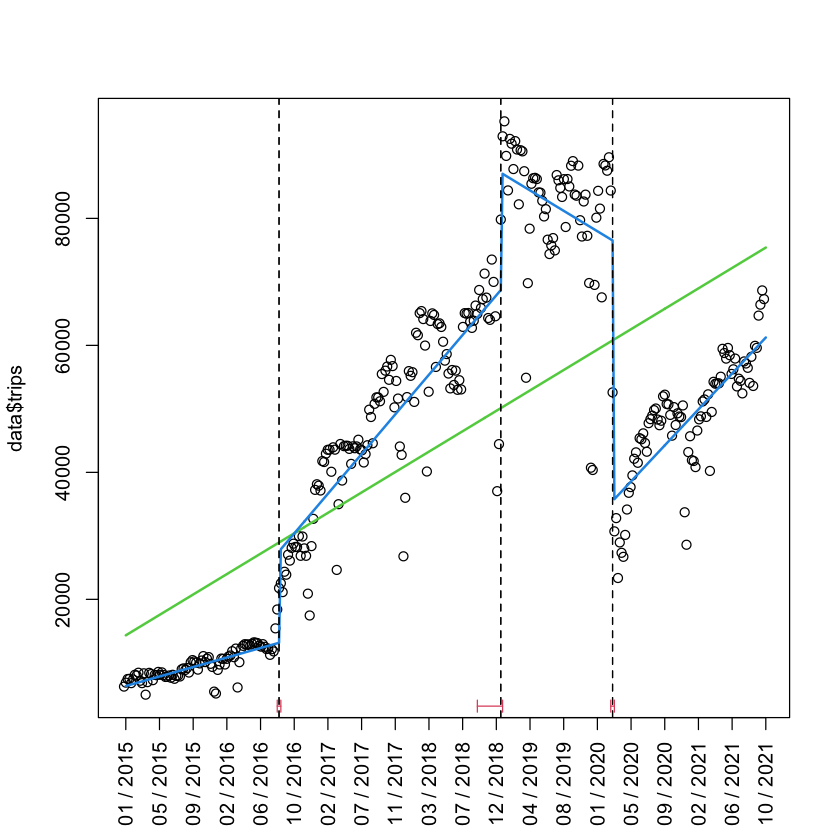
\includegraphics{/Users/jaimefco/Documents/AnalisisDeDatos/proyecto/plots/structChange_files/structChange_17_4.png}
\caption{}
\end{figure}

En rojo se observa el intervalo de confianza del punto de quiebre
utilizando el estadístico F. Para evaluar la calidad de nuestro modelos
de regresión, observamos el resumen que arroja R:

\begin{Shaded}
\begin{Highlighting}[]
\FunctionTok{summary}\NormalTok{(fm1)}
\end{Highlighting}
\end{Shaded}

\begin{verbatim}
Call:
lm(formula = trips ~ breakfactor(bp.bikes2)/date - 1, data = data)

Residuals:
   Min     1Q Median     3Q    Max
-37872  -1903    492   3757  16818

Coefficients:
                                      Estimate Std. Error t value Pr(>|t|)
breakfactor(bp.bikes2)segment1      -1.816e+05  6.812e+04  -2.666 0.008041 **
breakfactor(bp.bikes2)segment2      -7.867e+05  4.157e+04 -18.925  < 2e-16 ***
breakfactor(bp.bikes2)segment3       5.271e+05  1.205e+05   4.375  1.6e-05 ***
breakfactor(bp.bikes2)segment4      -7.583e+05  7.717e+04  -9.826  < 2e-16 ***
breakfactor(bp.bikes2)segment1:date  1.143e+01  4.070e+00   2.809 0.005249 **
breakfactor(bp.bikes2)segment2:date  4.780e+01  2.379e+00  20.089  < 2e-16 ***
breakfactor(bp.bikes2)segment3:date -2.458e+01  6.649e+00  -3.697 0.000254 ***
breakfactor(bp.bikes2)segment4:date  4.330e+01  4.142e+00  10.455  < 2e-16 ***
---
Signif. codes:  0 ‘***’ 0.001 ‘**’ 0.01 ‘*’ 0.05 ‘.’ 0.1 ‘ ’ 1

Residual standard error: 6558 on 348 degrees of freedom
Multiple R-squared:  0.9842,	Adjusted R-squared:  0.9838
F-statistic:  2711 on 8 and 348 DF,  p-value: < 2.2e-16
\end{verbatim}

Vemos que el p-valor del estadístico \(T\) para cada coeficiente es muy
bajo, menor a \(10^{-3}\) en la mayoría de los casos. Además vemos que
\(R^2\) es muy cercano a 1, lo que habla muy bien de nuestro modelos.

Por último graficamos la serie de tiempo, en rojo los modelos de
regresión lineal para cada intervalo, en verde el modelo lineal ajustado
a toda la serie y en en rojo las fechas estimadas de los puntos de
quiebre.

\begin{figure}
\centering
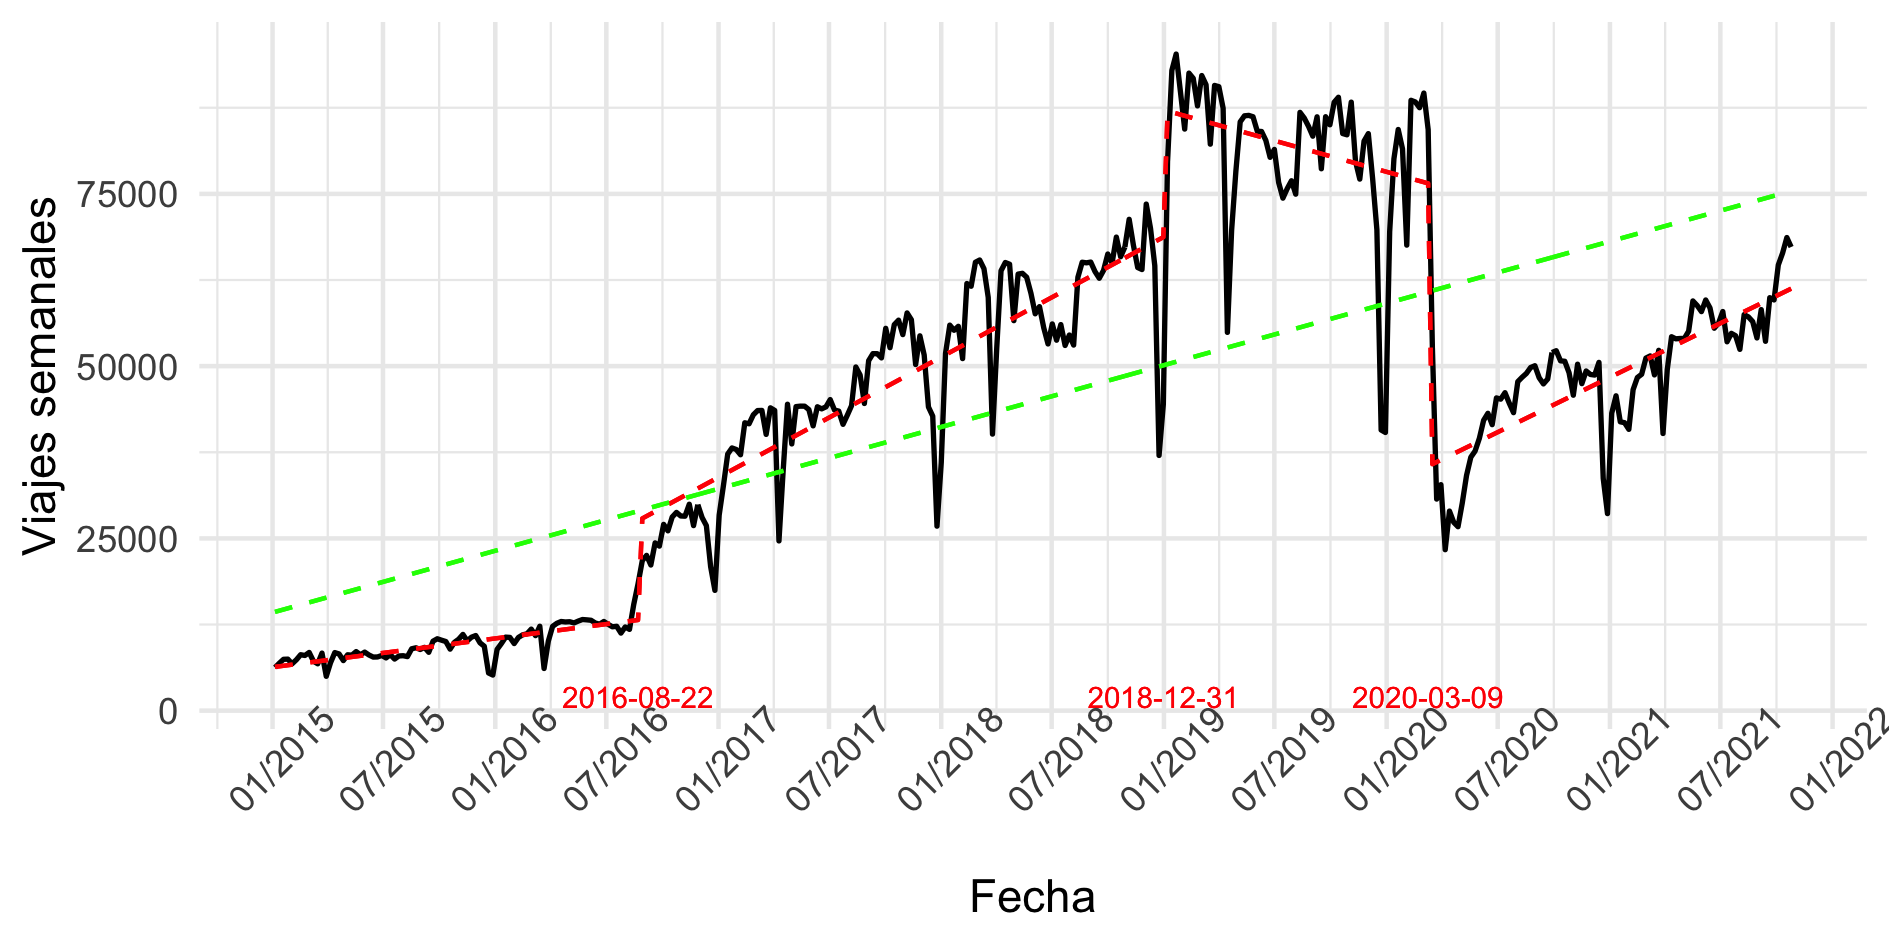
\includegraphics{/Users/jaimefco/Documents/AnalisisDeDatos/proyecto/plots/serie_breaks.png}
\caption{}
\end{figure}

¿A qué se pueden deber los puntos de quiebre?

Tratando de explicar los cambios de estructura, nos dimos a la tarea de
investigar noticias relativas al programa Mi Bici en fechas cercanas a
los puntos de quiebre. Los resultados fueron los siguientes:

\begin{itemize}
\item
  El octubre de 2016 se
  \href{https://www.informador.mx/Jalisco/Inauguran-segunda-etapa-de-MiBici-20161027-0035.html}{inauguró
  la segunda etapa del programa}, con la ampliación del número de
  estaciones.
\item
  En noviembre de 2018 se
  \href{https://www.eloccidental.com.mx/local/inauguran-tercera-etapa-de-mibici-2714371.html}{inauguró
  la tercera etapa del programa}.
\item
  El 3 de marzo de 2020 se
  \href{https://www.animalpolitico.com/2020/03/jalisco-suspende-clases-universidades-eventos-masivos-coronavirus/}{suspendieron
  las clases presenciales} en el estado de Jalisco.
\end{itemize}

Salvo la suspensión de clases, los punto de quiebre no corresponden
exactamente a las inauguraciones del número de estaciones, pero están
fuertemente relacionadas pues, de acuerdo a los datos reportados, las
estaciones ya se encontraban en uso semanas antes de la inauguración.
Como ejemplo, la semana del 15 de agosoto de 2016 se dio una apliación
de aproximadamente 120 a 234 estaciones en uso. Como comparación, en el
análsis localizamos un punto de quiebre en la semana del 22 de agosoto
del mismo año.

En el siguiente capítulo se abarca un poco más a detalle el impacto en
la ampliación del número de estaciones.

\begin{center}\rule{0.5\linewidth}{0.5pt}\end{center}

\hypertarget{anuxe1lisis-de-las-estaciones}{%
\subsection{Análisis de las
estaciones}\label{anuxe1lisis-de-las-estaciones}}

En esta sección exploramos los viajes entre puntos de recogida de
bicicletas, puntos a los que llamaremos estaciones. La idea surge de las
observaciones de que hay un comportamiento diferente a partir de la
apertura de nuevas estaciones. Para poder hacer observaciones nos
apoyamos en herramientas de \emph{R} así como de \emph{Python}.

Se tomó el acumulado de viajes mensuales y con ello se generaron
matrices con la siguiente cualidad:\\
\textbf{Si había un viaje de la estación \emph{i} hacia la estación
\emph{j} entonces a la entrada \emph{(i,j)} de la matriz se le suma 1.}

La siguiente gráfica muestra la cantidad de diferentes estaciones que
registraron viajes semanalmente.

\begin{figure}
\centering
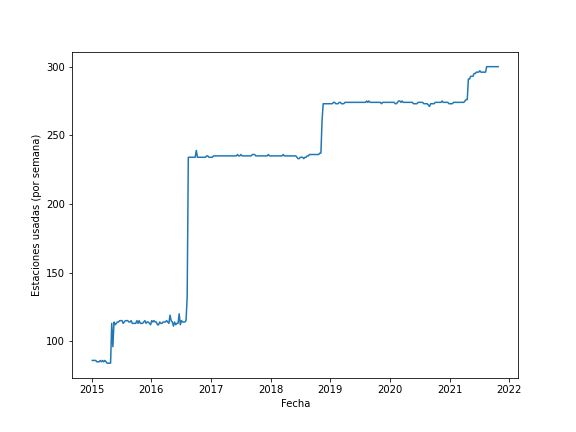
\includegraphics{/Users/jaimefco/Documents/AnalisisDeDatos/proyecto/plots/stations_weekly.png}
\caption{}
\end{figure}

Observemos que hay 4 aumentos importantes en cuanto a la cantidad de
estaciones diferentes, por ello exploramos como se se comporta la
interacción en estas etapas.

En las gráficas tipo HeatMap se muestra la interacción de viajes, donde
oscuro significa nula o casi nula interacción. Cada una de ellas fue
calculada promediando las interacciones mensuales de acuerdo a la
duración de la etapa.

\begin{figure}
\centering
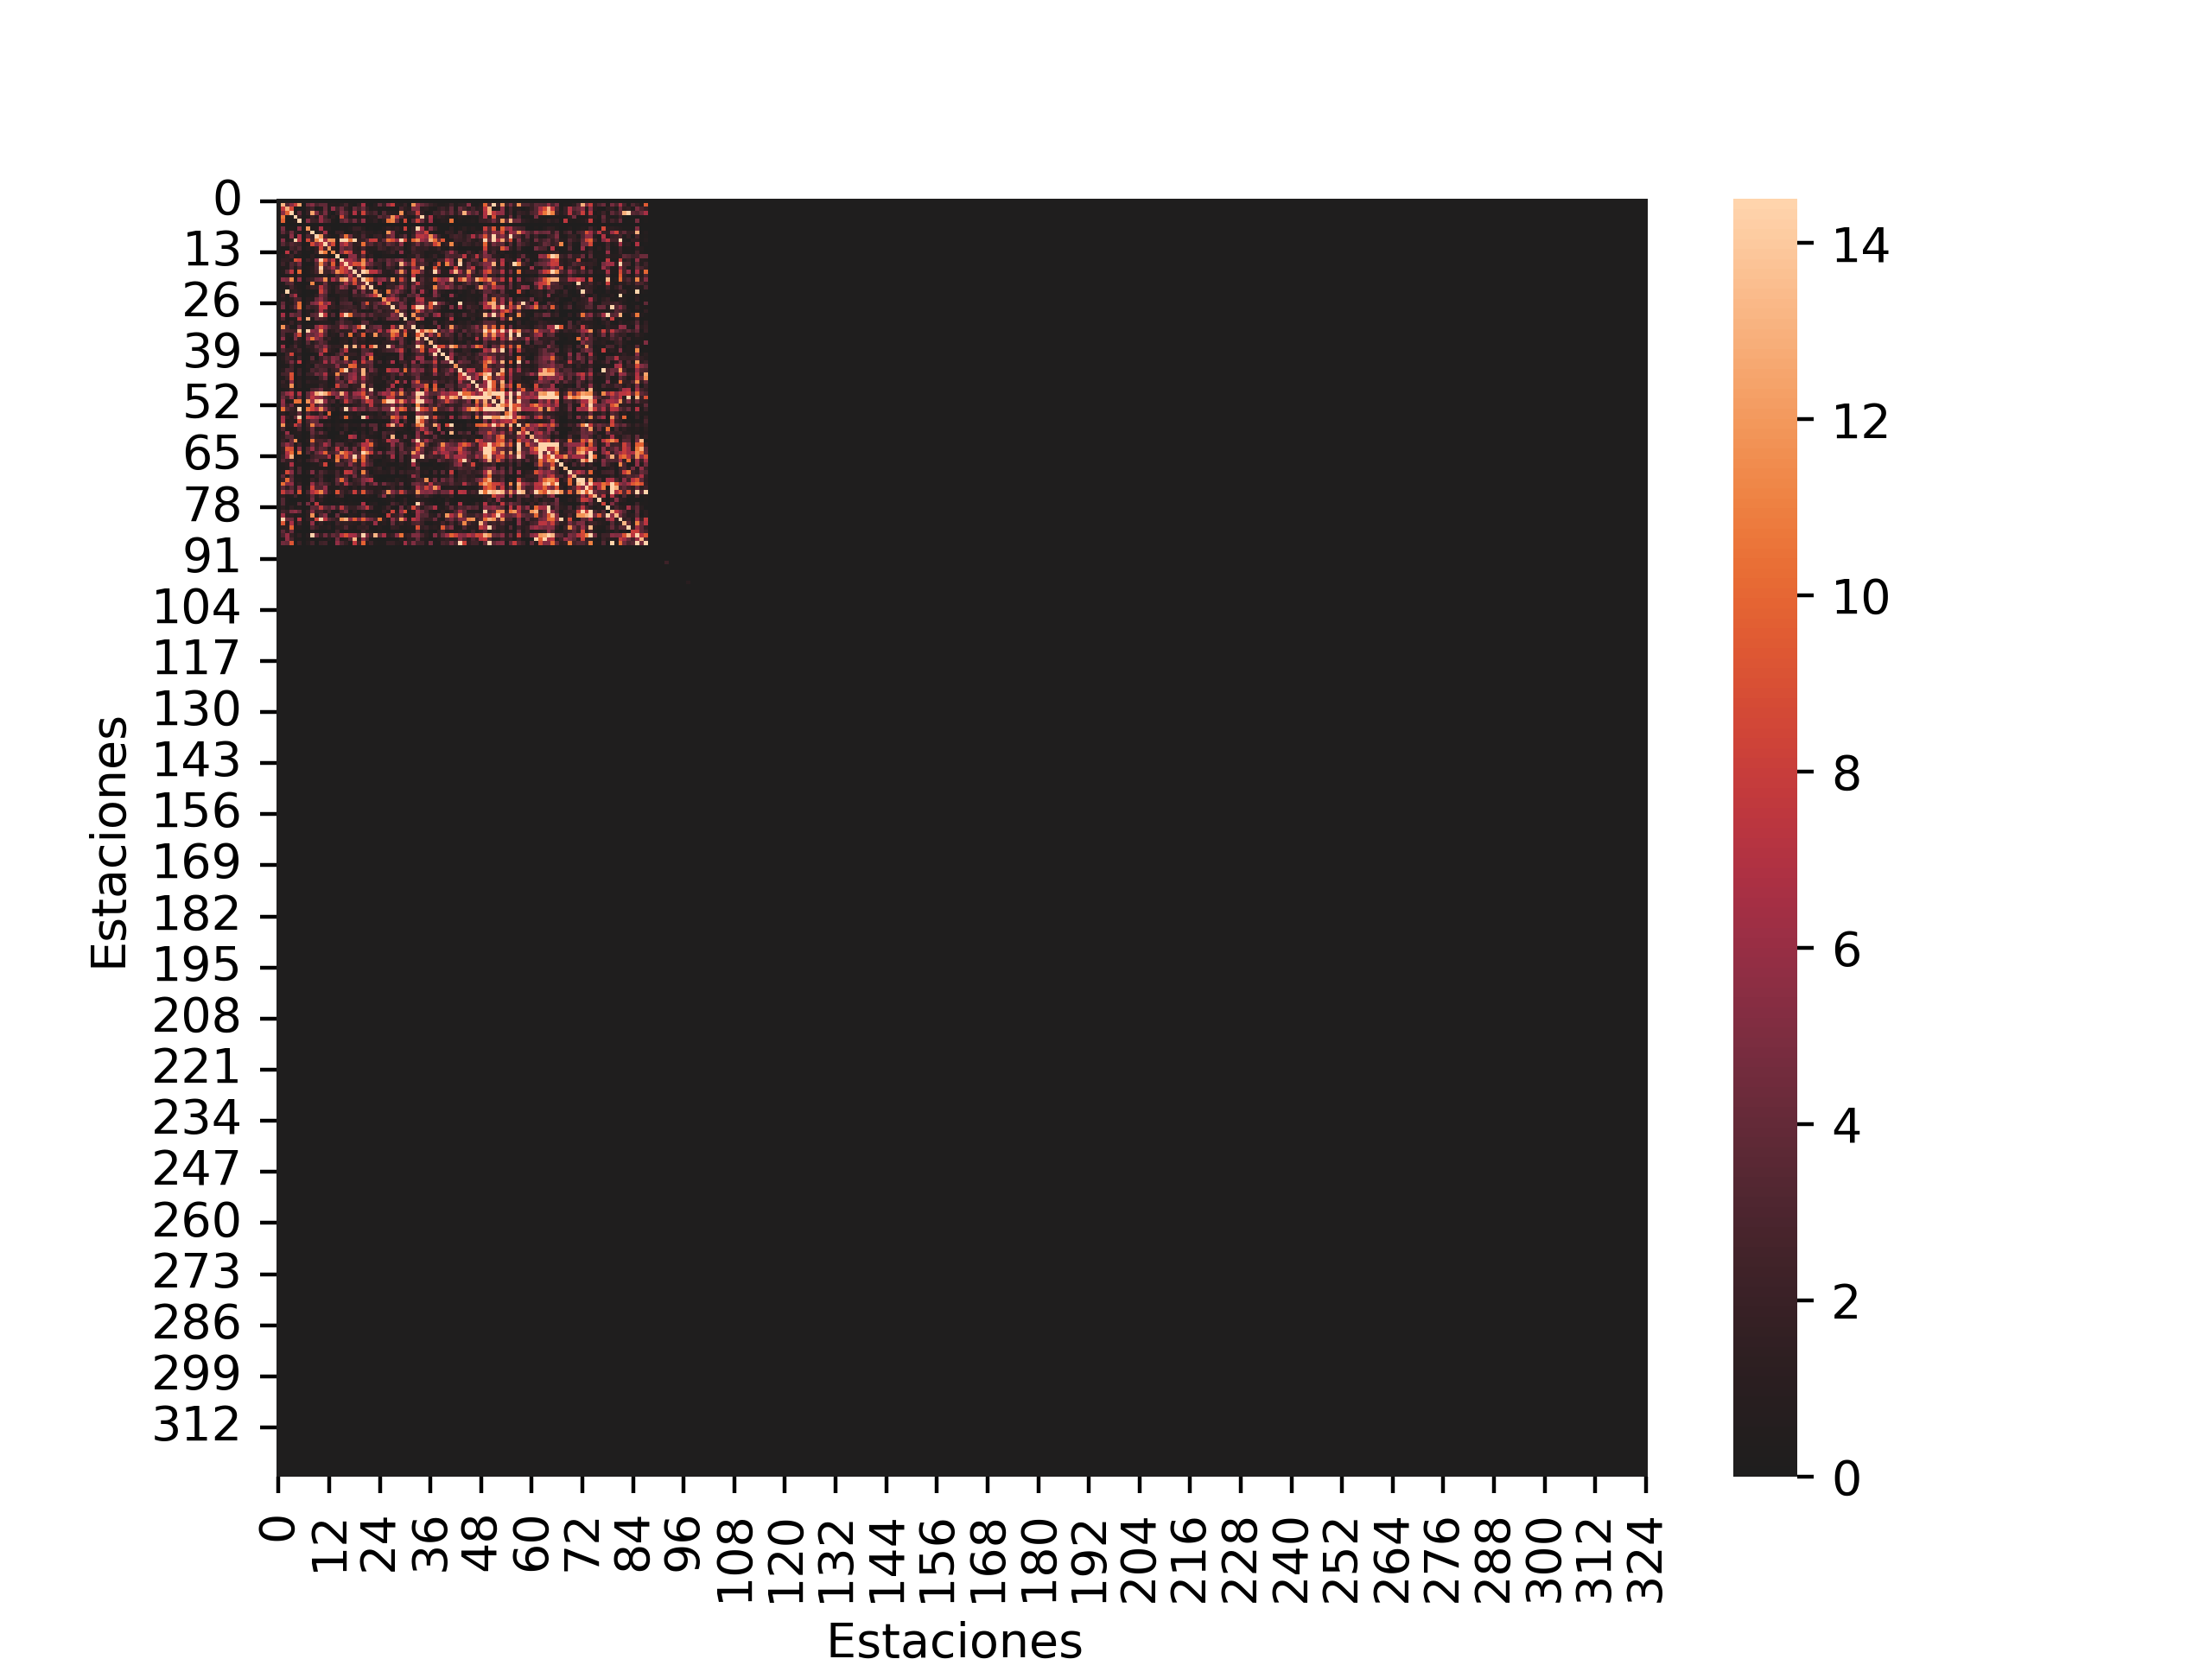
\includegraphics{/Users/jaimefco/Documents/AnalisisDeDatos/proyecto/plots/resultsUno.png}
\caption{Etapa 1}
\end{figure}

Etapa Uno tomando los primeros 4 meses del registro, de Enero de 2015 a
Abril de 2015.

\begin{figure}
\centering
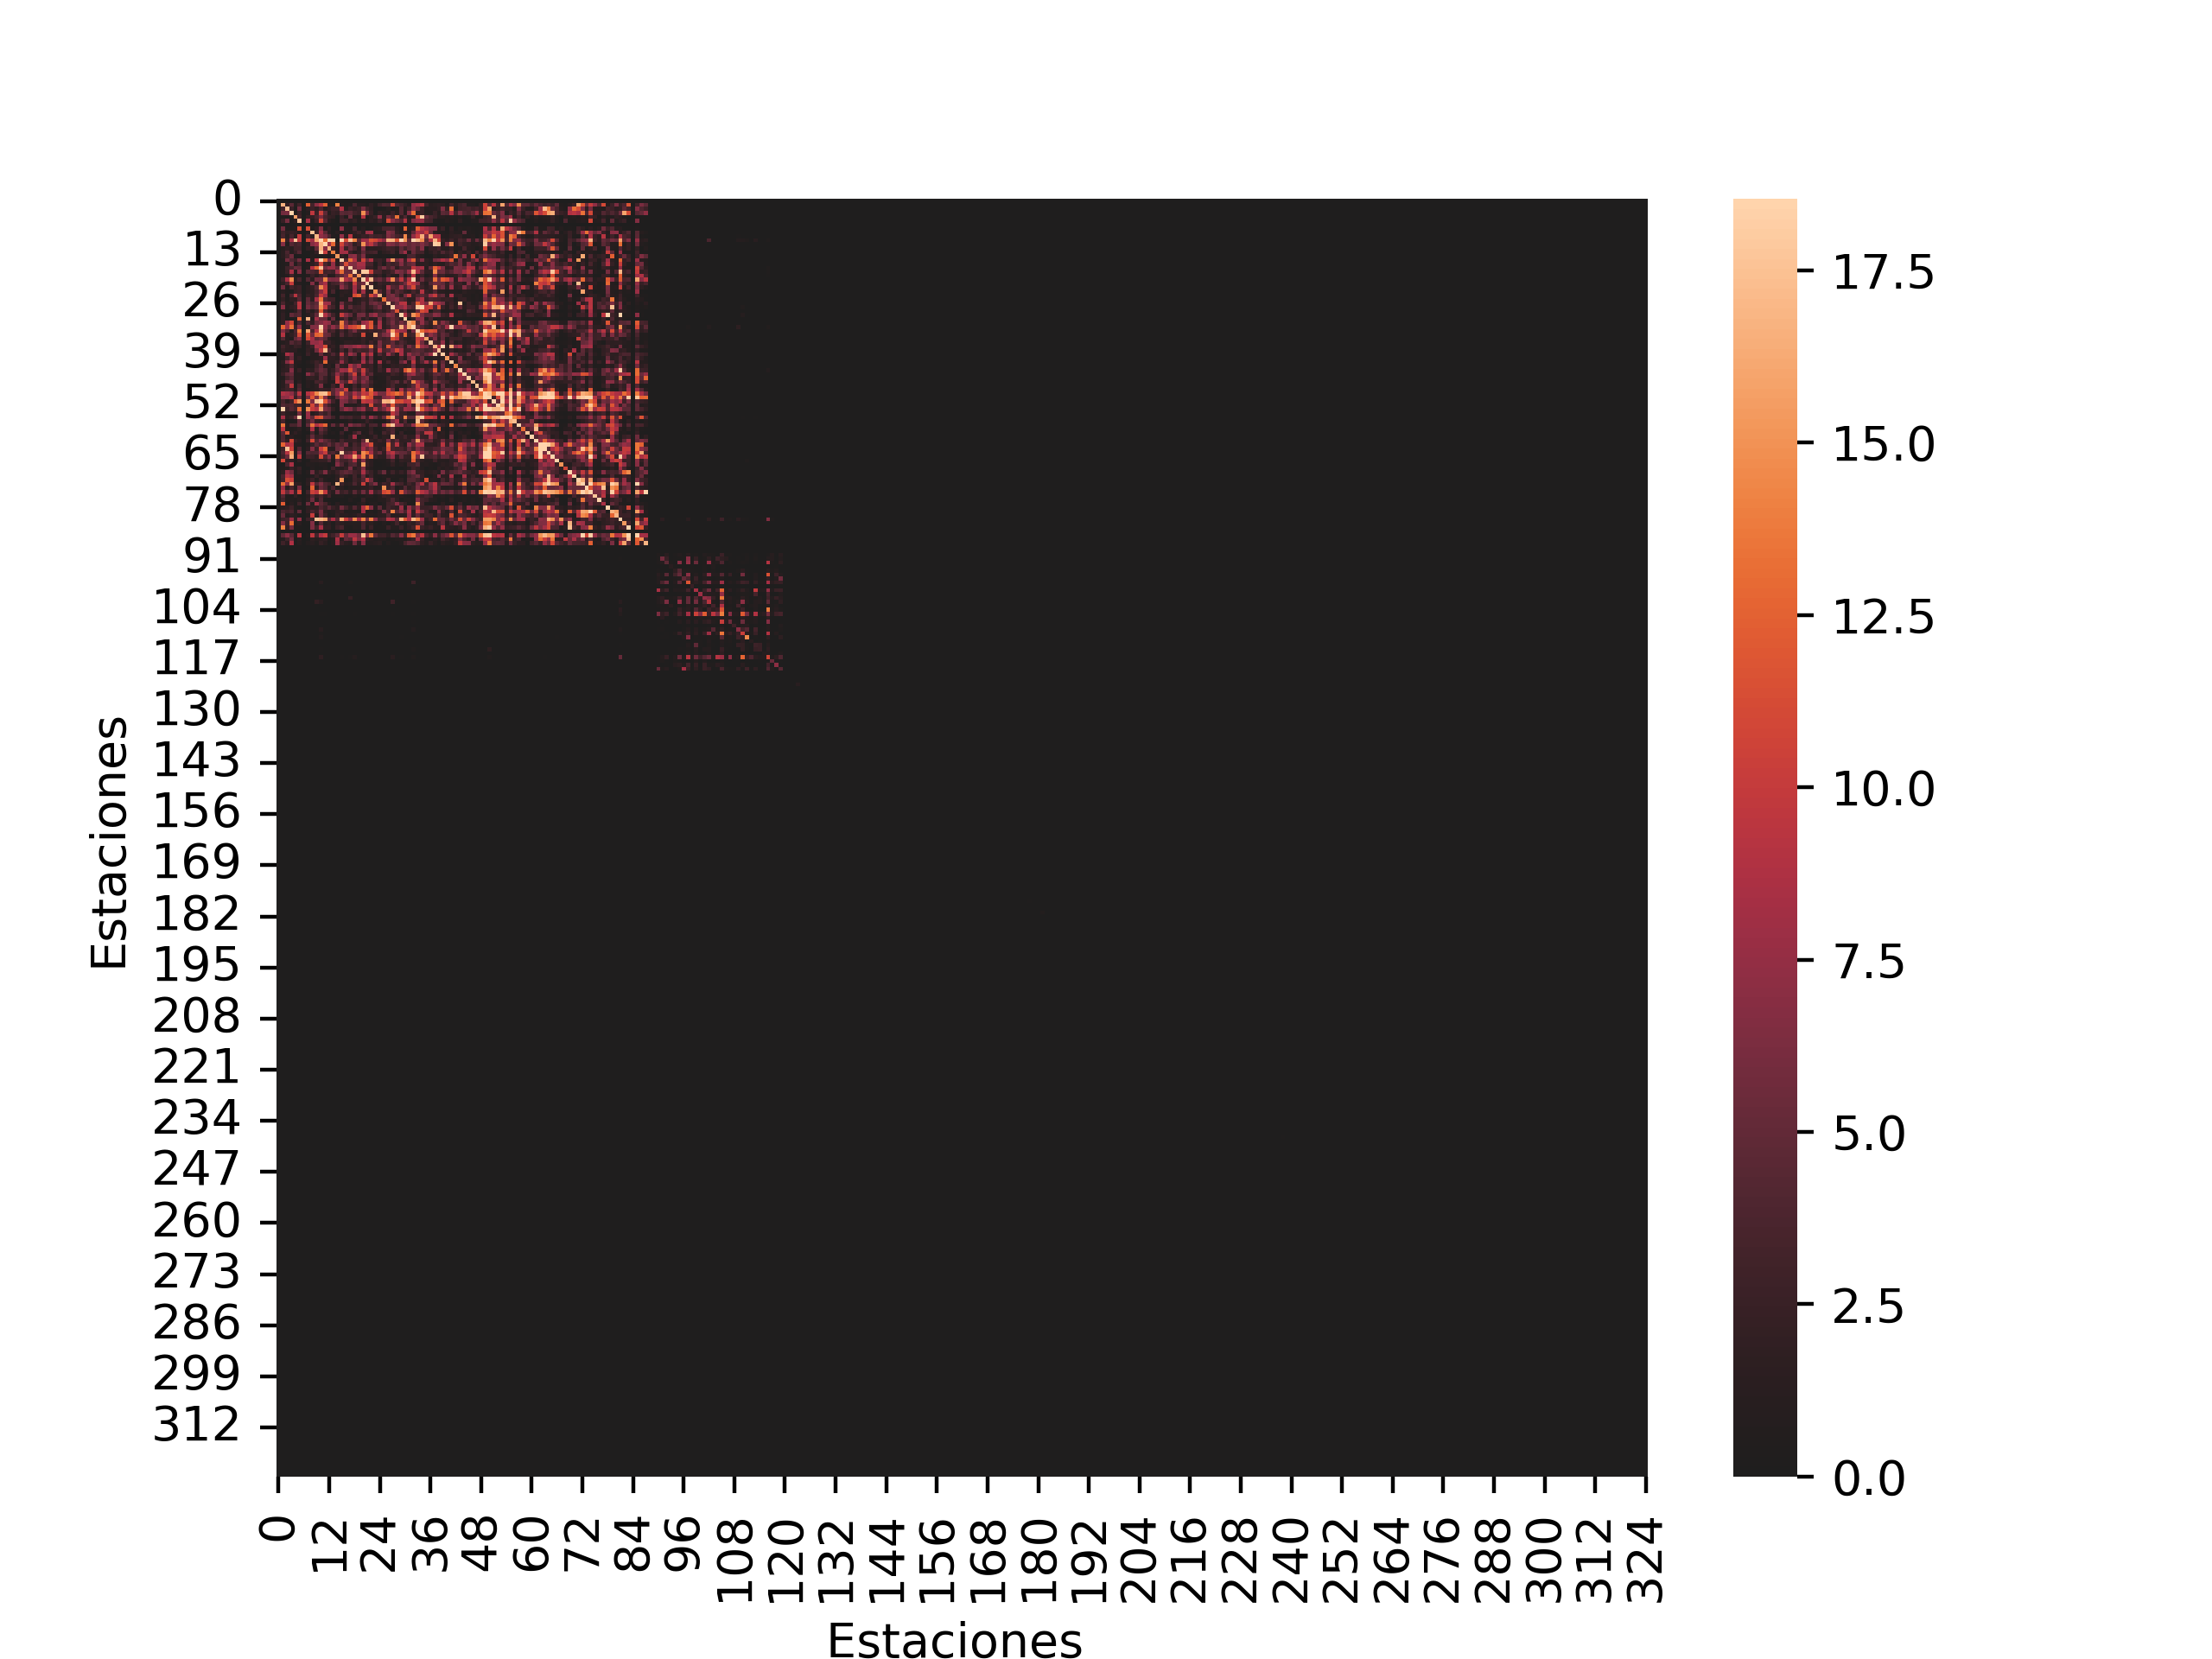
\includegraphics{/Users/jaimefco/Documents/AnalisisDeDatos/proyecto/plots/resultsDos.png}
\caption{Etapa 2}
\end{figure}

Etapa Dos tomando de Mayo de 2015 a Julio de 2016.

Podemos observar que la primera ampliación no causa un gran inmpacto y
las estaciones agregadas no tienen mucha interacción con las estaciones
iniciales, pues al agregarse no se nota un cambio visible en el mapa de
calor.

\begin{figure}
\centering
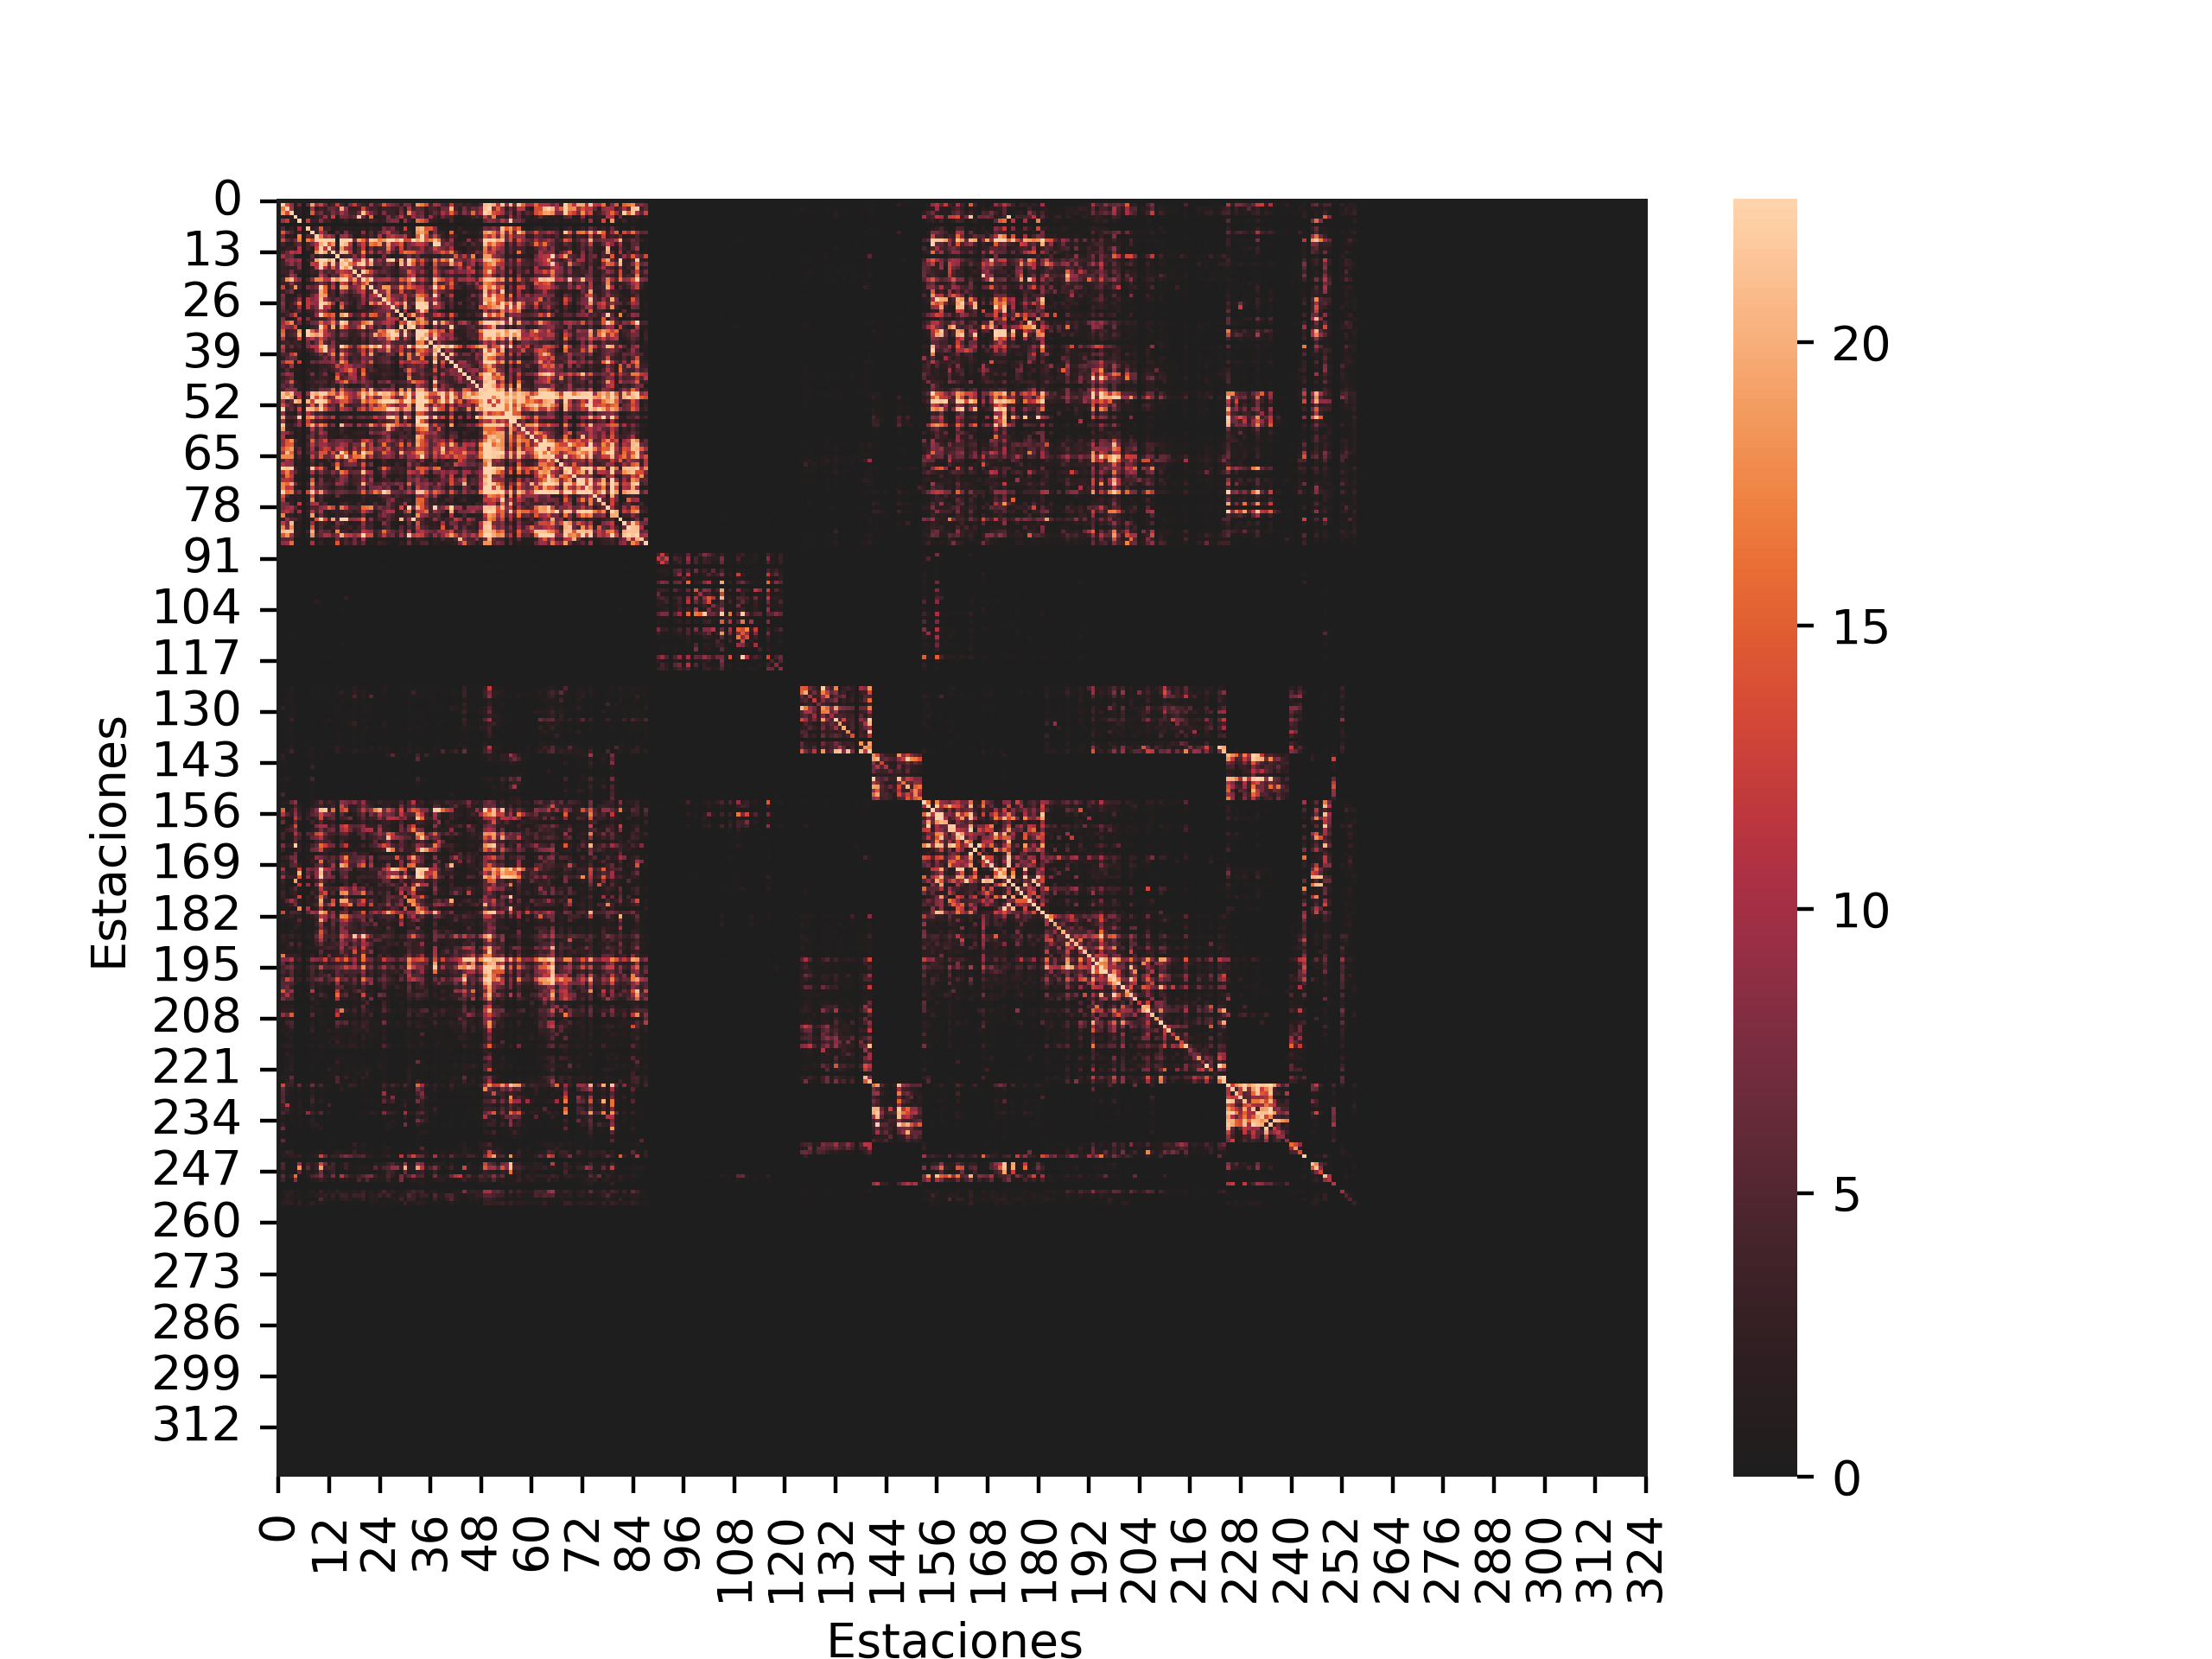
\includegraphics{/Users/jaimefco/Documents/AnalisisDeDatos/proyecto/plots/resultsTres.png}
\caption{Etapa 3}
\end{figure}

Etapa Tres tomando de Agosto de 2016 a Octubre de 2018.

Después de la segunda ampliación se observa un claro incremento en la
actividad, no solo entre las nuevas estaciones, sino también con las
estaciones de la primera estapa pues se nota una iluminación en los
puntos correspondientes a esta comunicación. También hay un incremento
en las cantidas de viajes entre estaciones, lo que sugiere que
incrementó la actividad en general, podemos asumir que hay evidencia
visual de que en esta ampliación hubo un cambio significativo en las
cantidades de viajes en general.

\begin{figure}
\centering
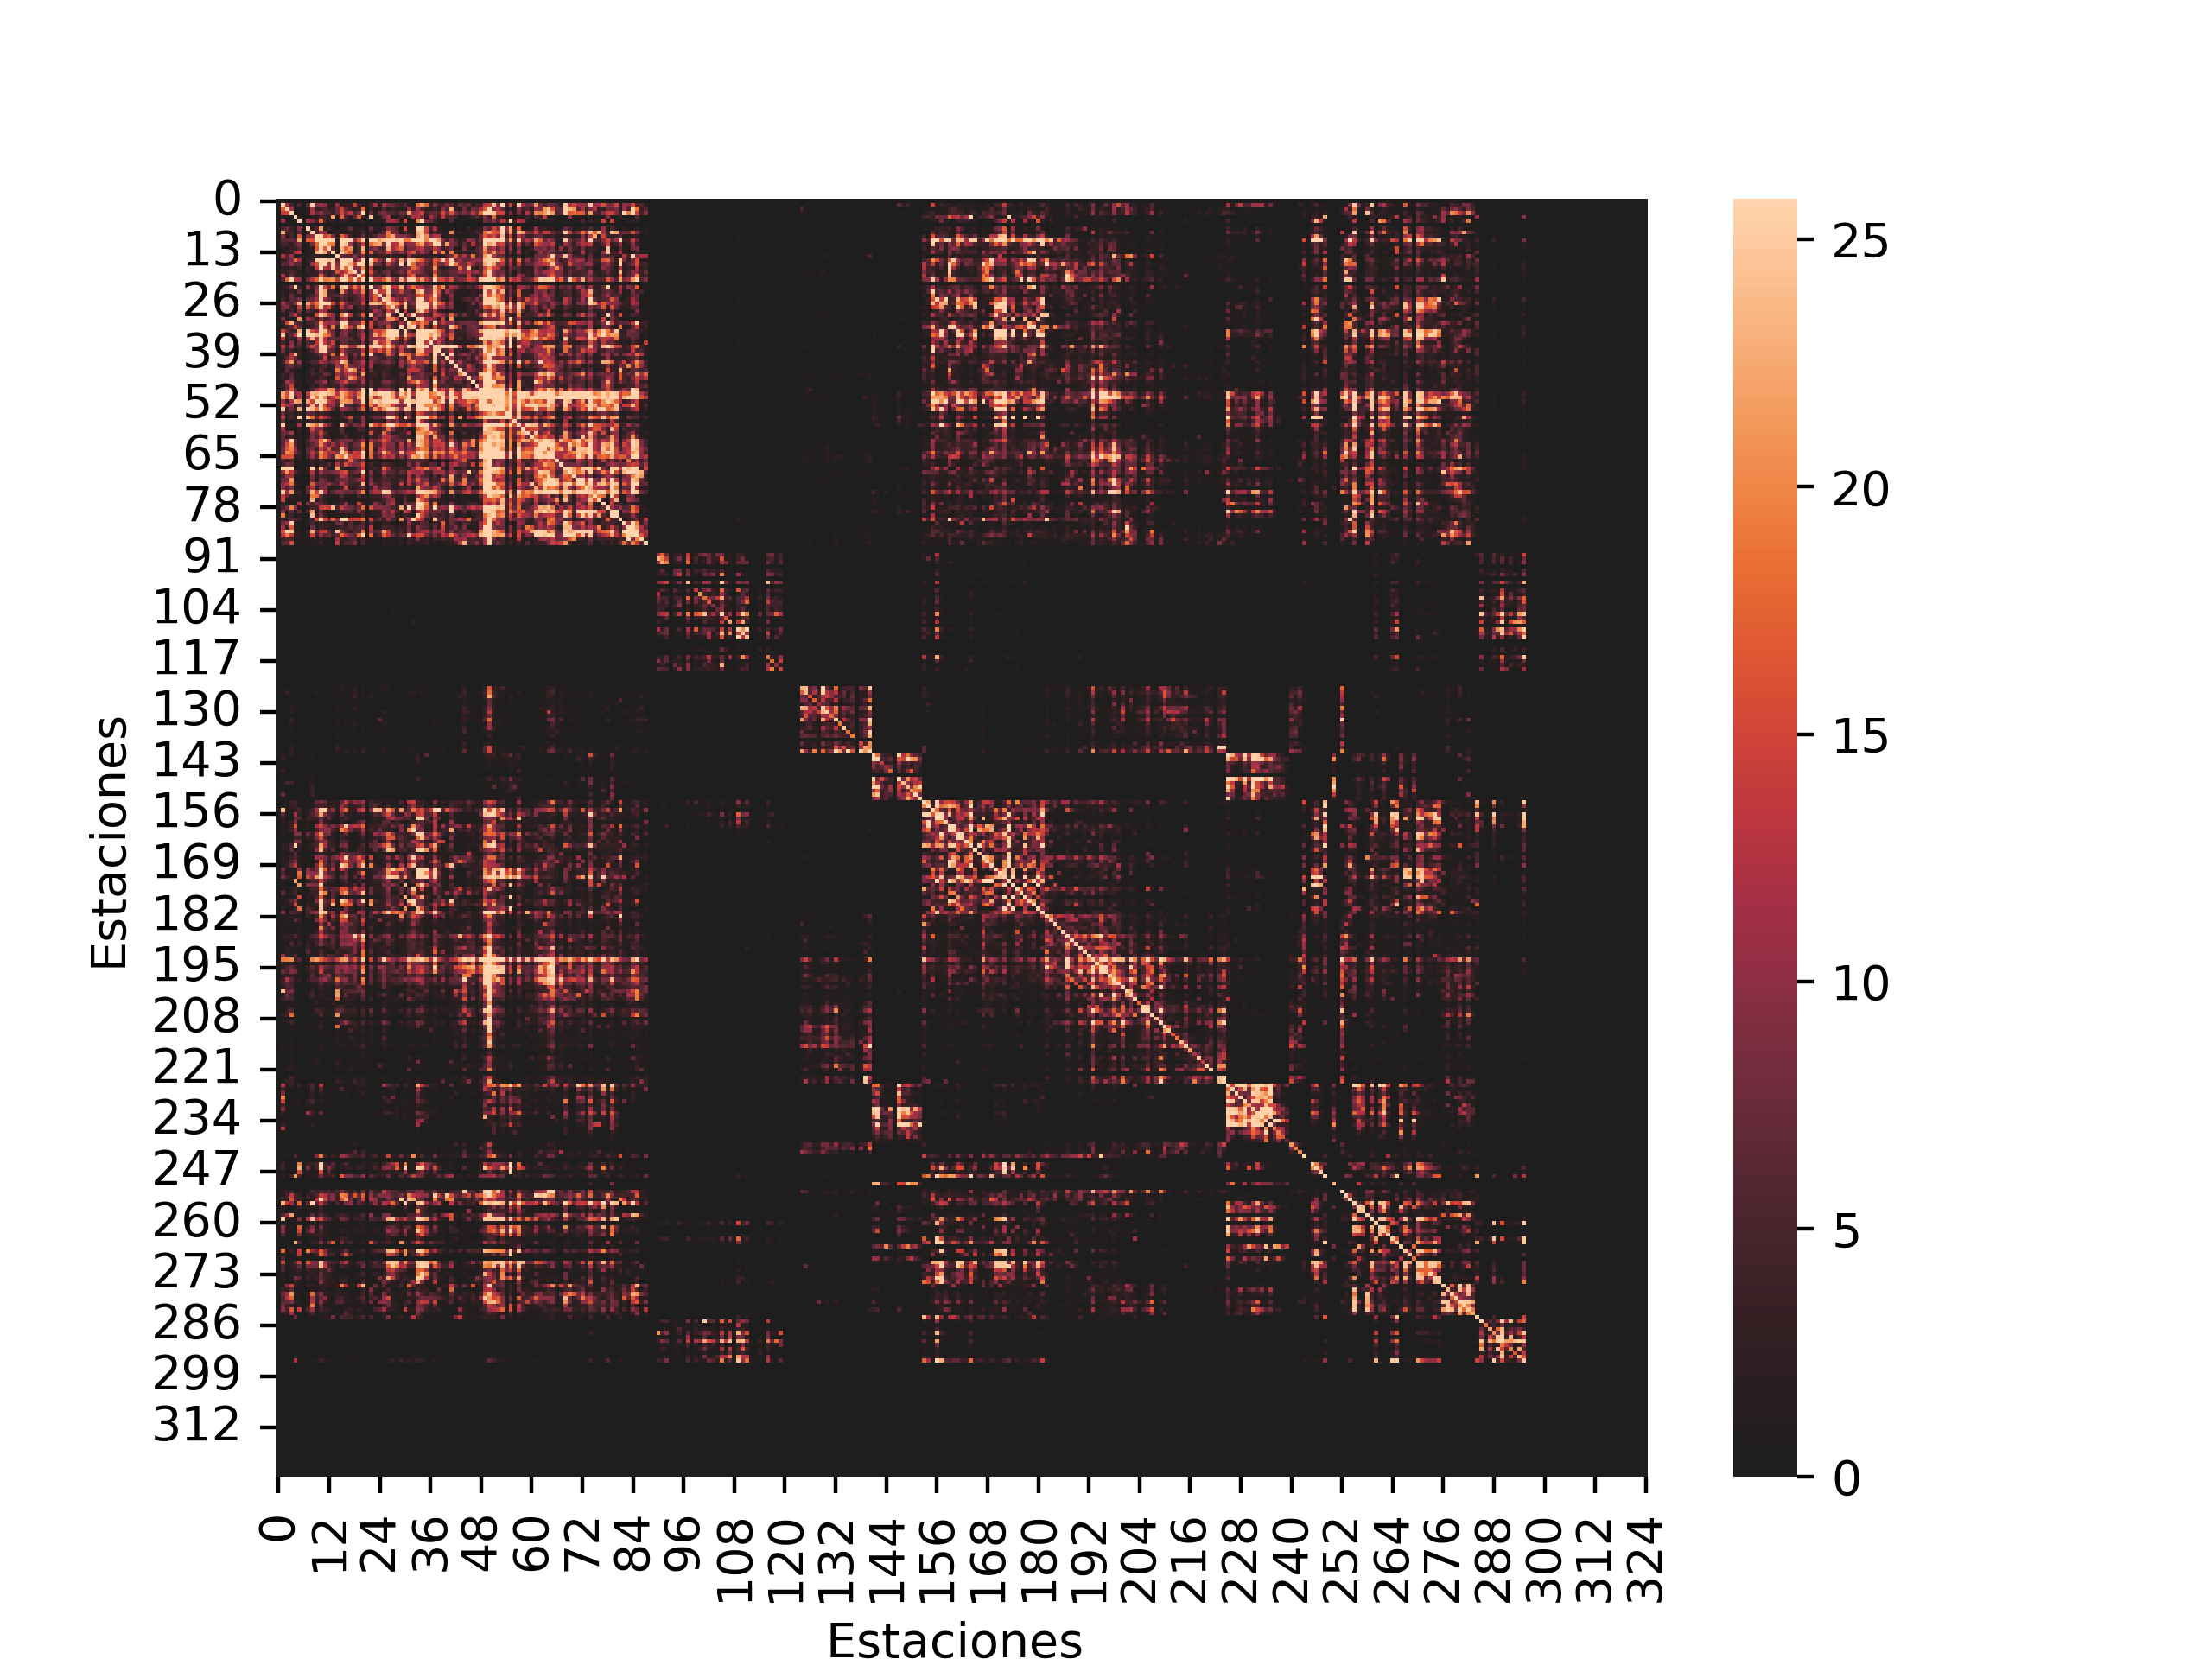
\includegraphics{/Users/jaimefco/Documents/AnalisisDeDatos/proyecto/plots/resultsCuatro.png}
\caption{Etapa 4}
\end{figure}

Etapa Cuatro tomando de Noviembre de 2018 a Febrero de 2020.

Decidimos hacer un corte aquí por el evento del confinamiento dictado a
inicios de Marzo de 2020.

\begin{figure}
\centering
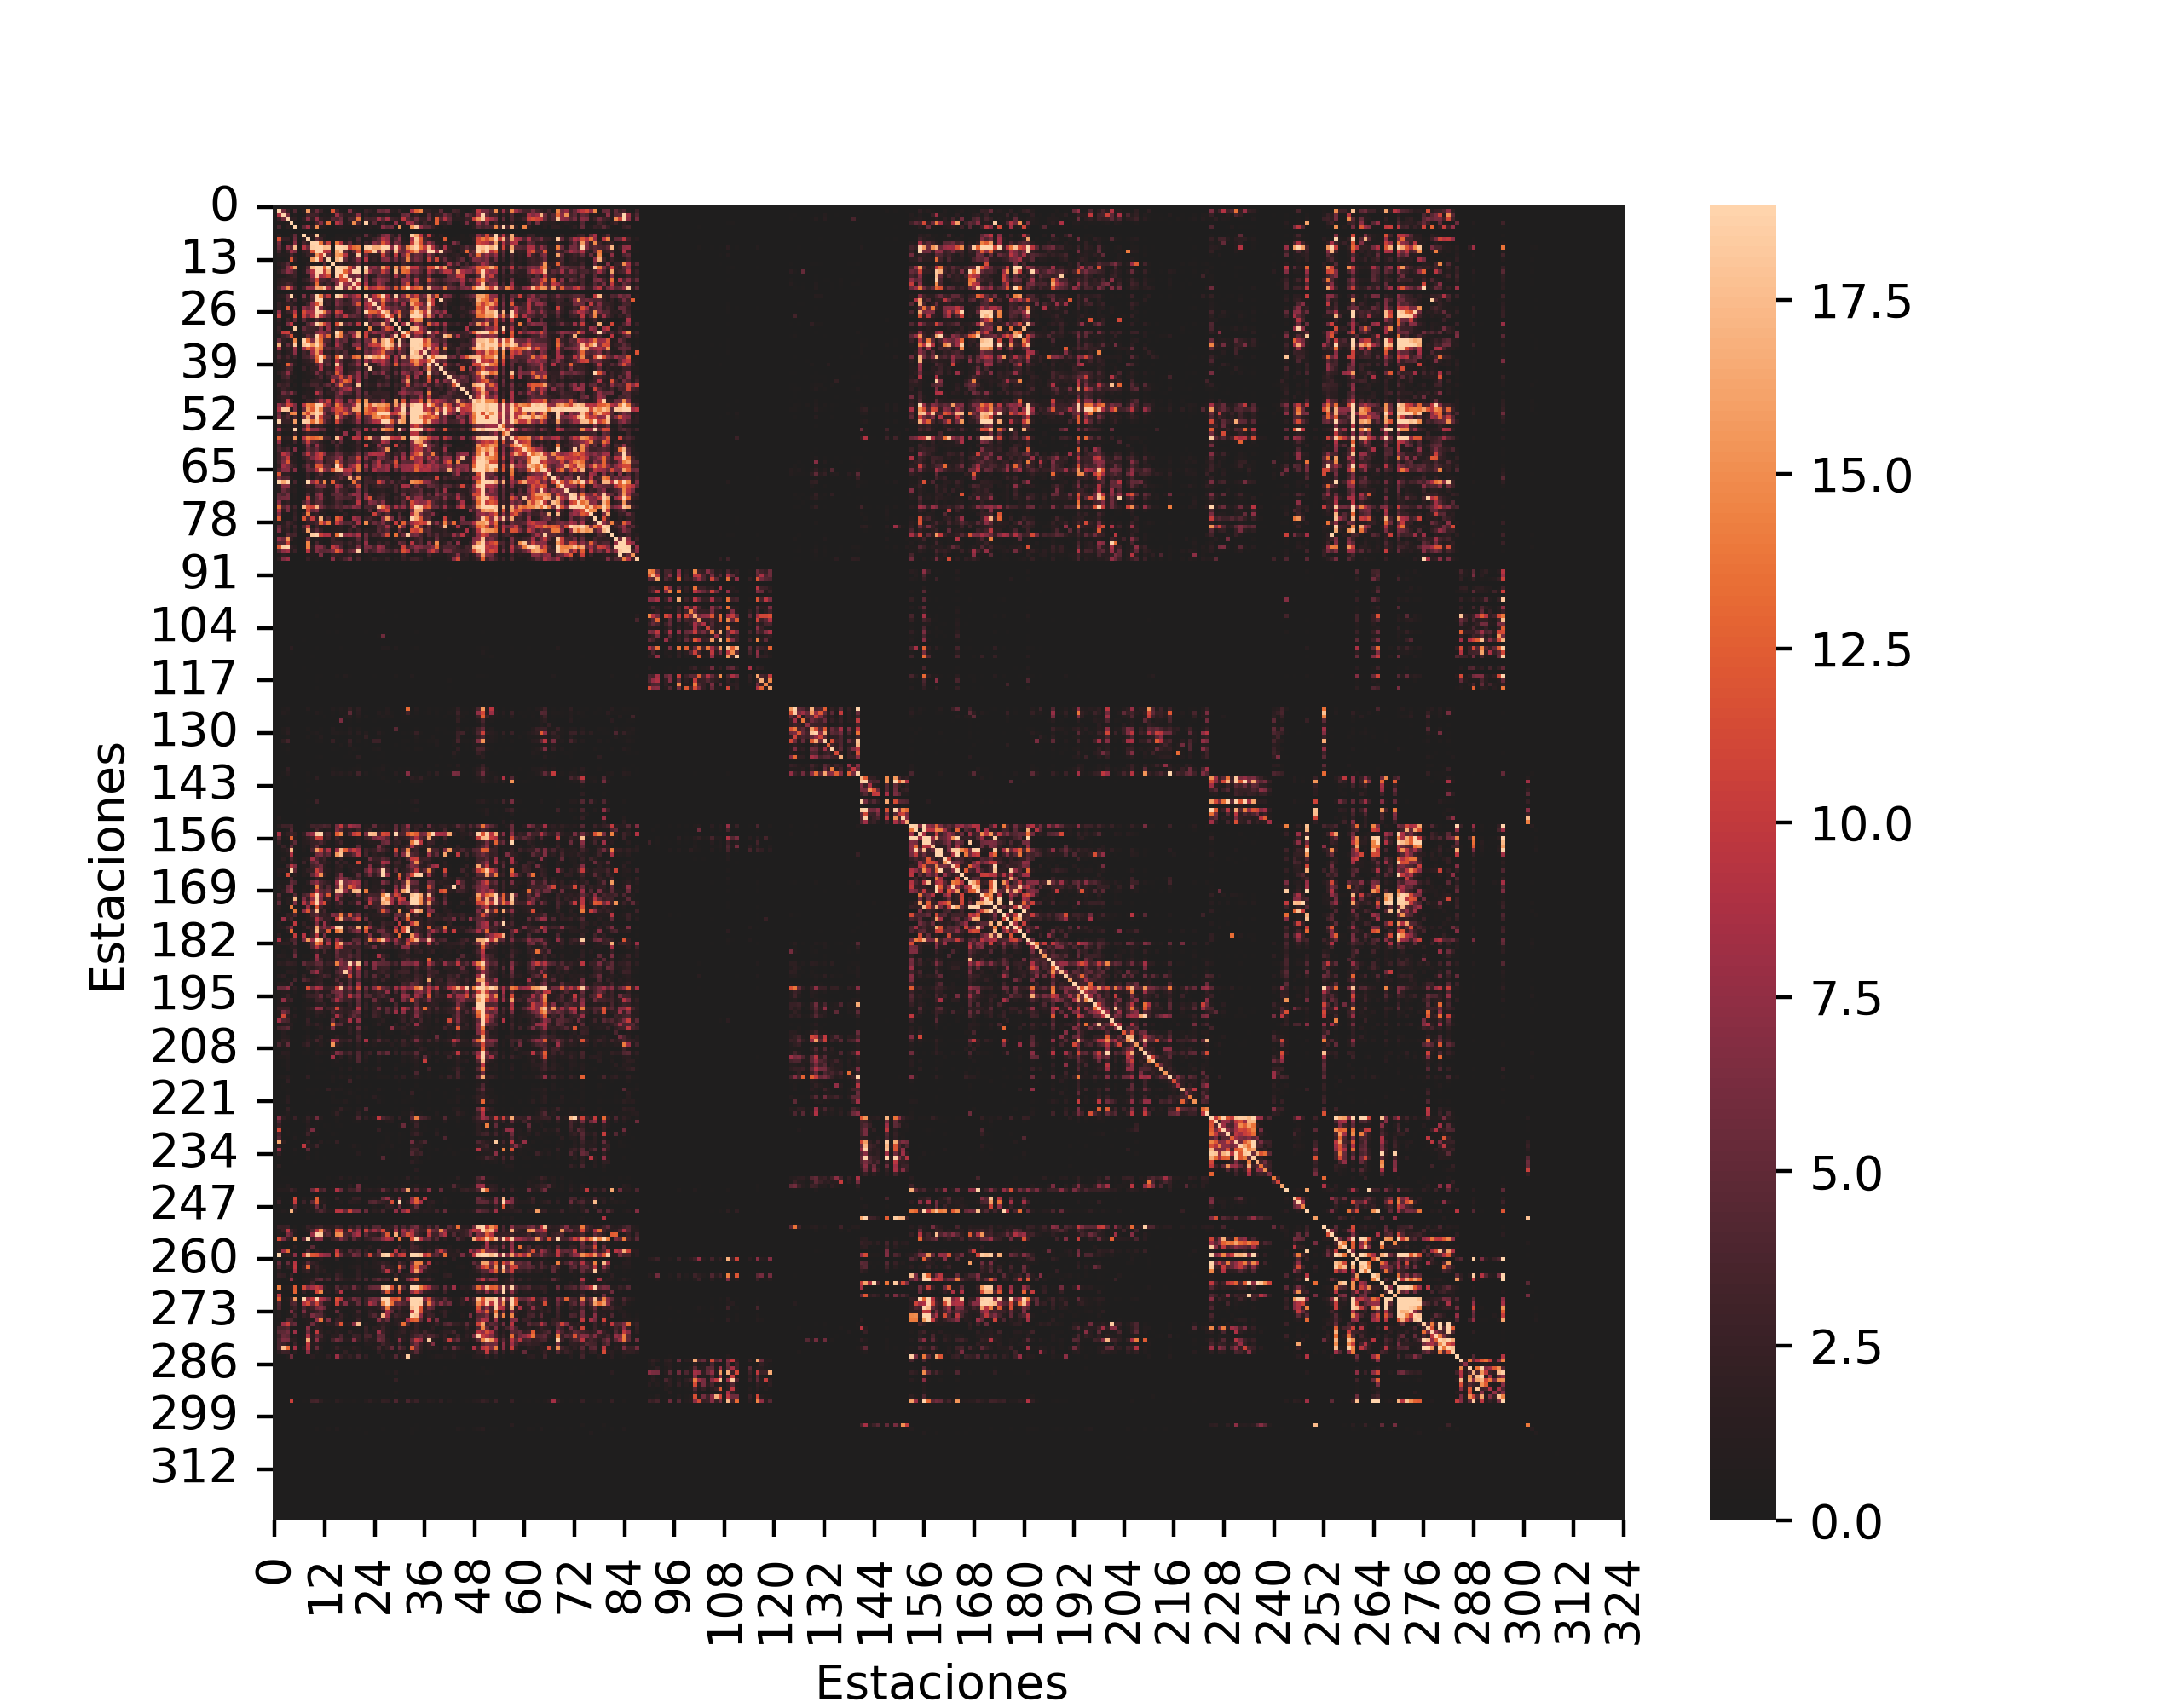
\includegraphics{/Users/jaimefco/Documents/AnalisisDeDatos/proyecto/plots/resultsCinco.png}
\caption{Etapa 5}
\end{figure}

Etapa Cinco tomando de Marzo de 2020 a Abril de 2021.

Después de la tercera ampliación, podemos ver que no hay un gran cambio
entre el comportamiento de las estaciones anteriores, sin embargo si hay
un nuevo aporte pues las estaciones agregadas en esta etapa tienen
intereacción con las estaciones antiguas, pero casi nula con las
estaciones de la segunda etapa.

\begin{figure}
\centering
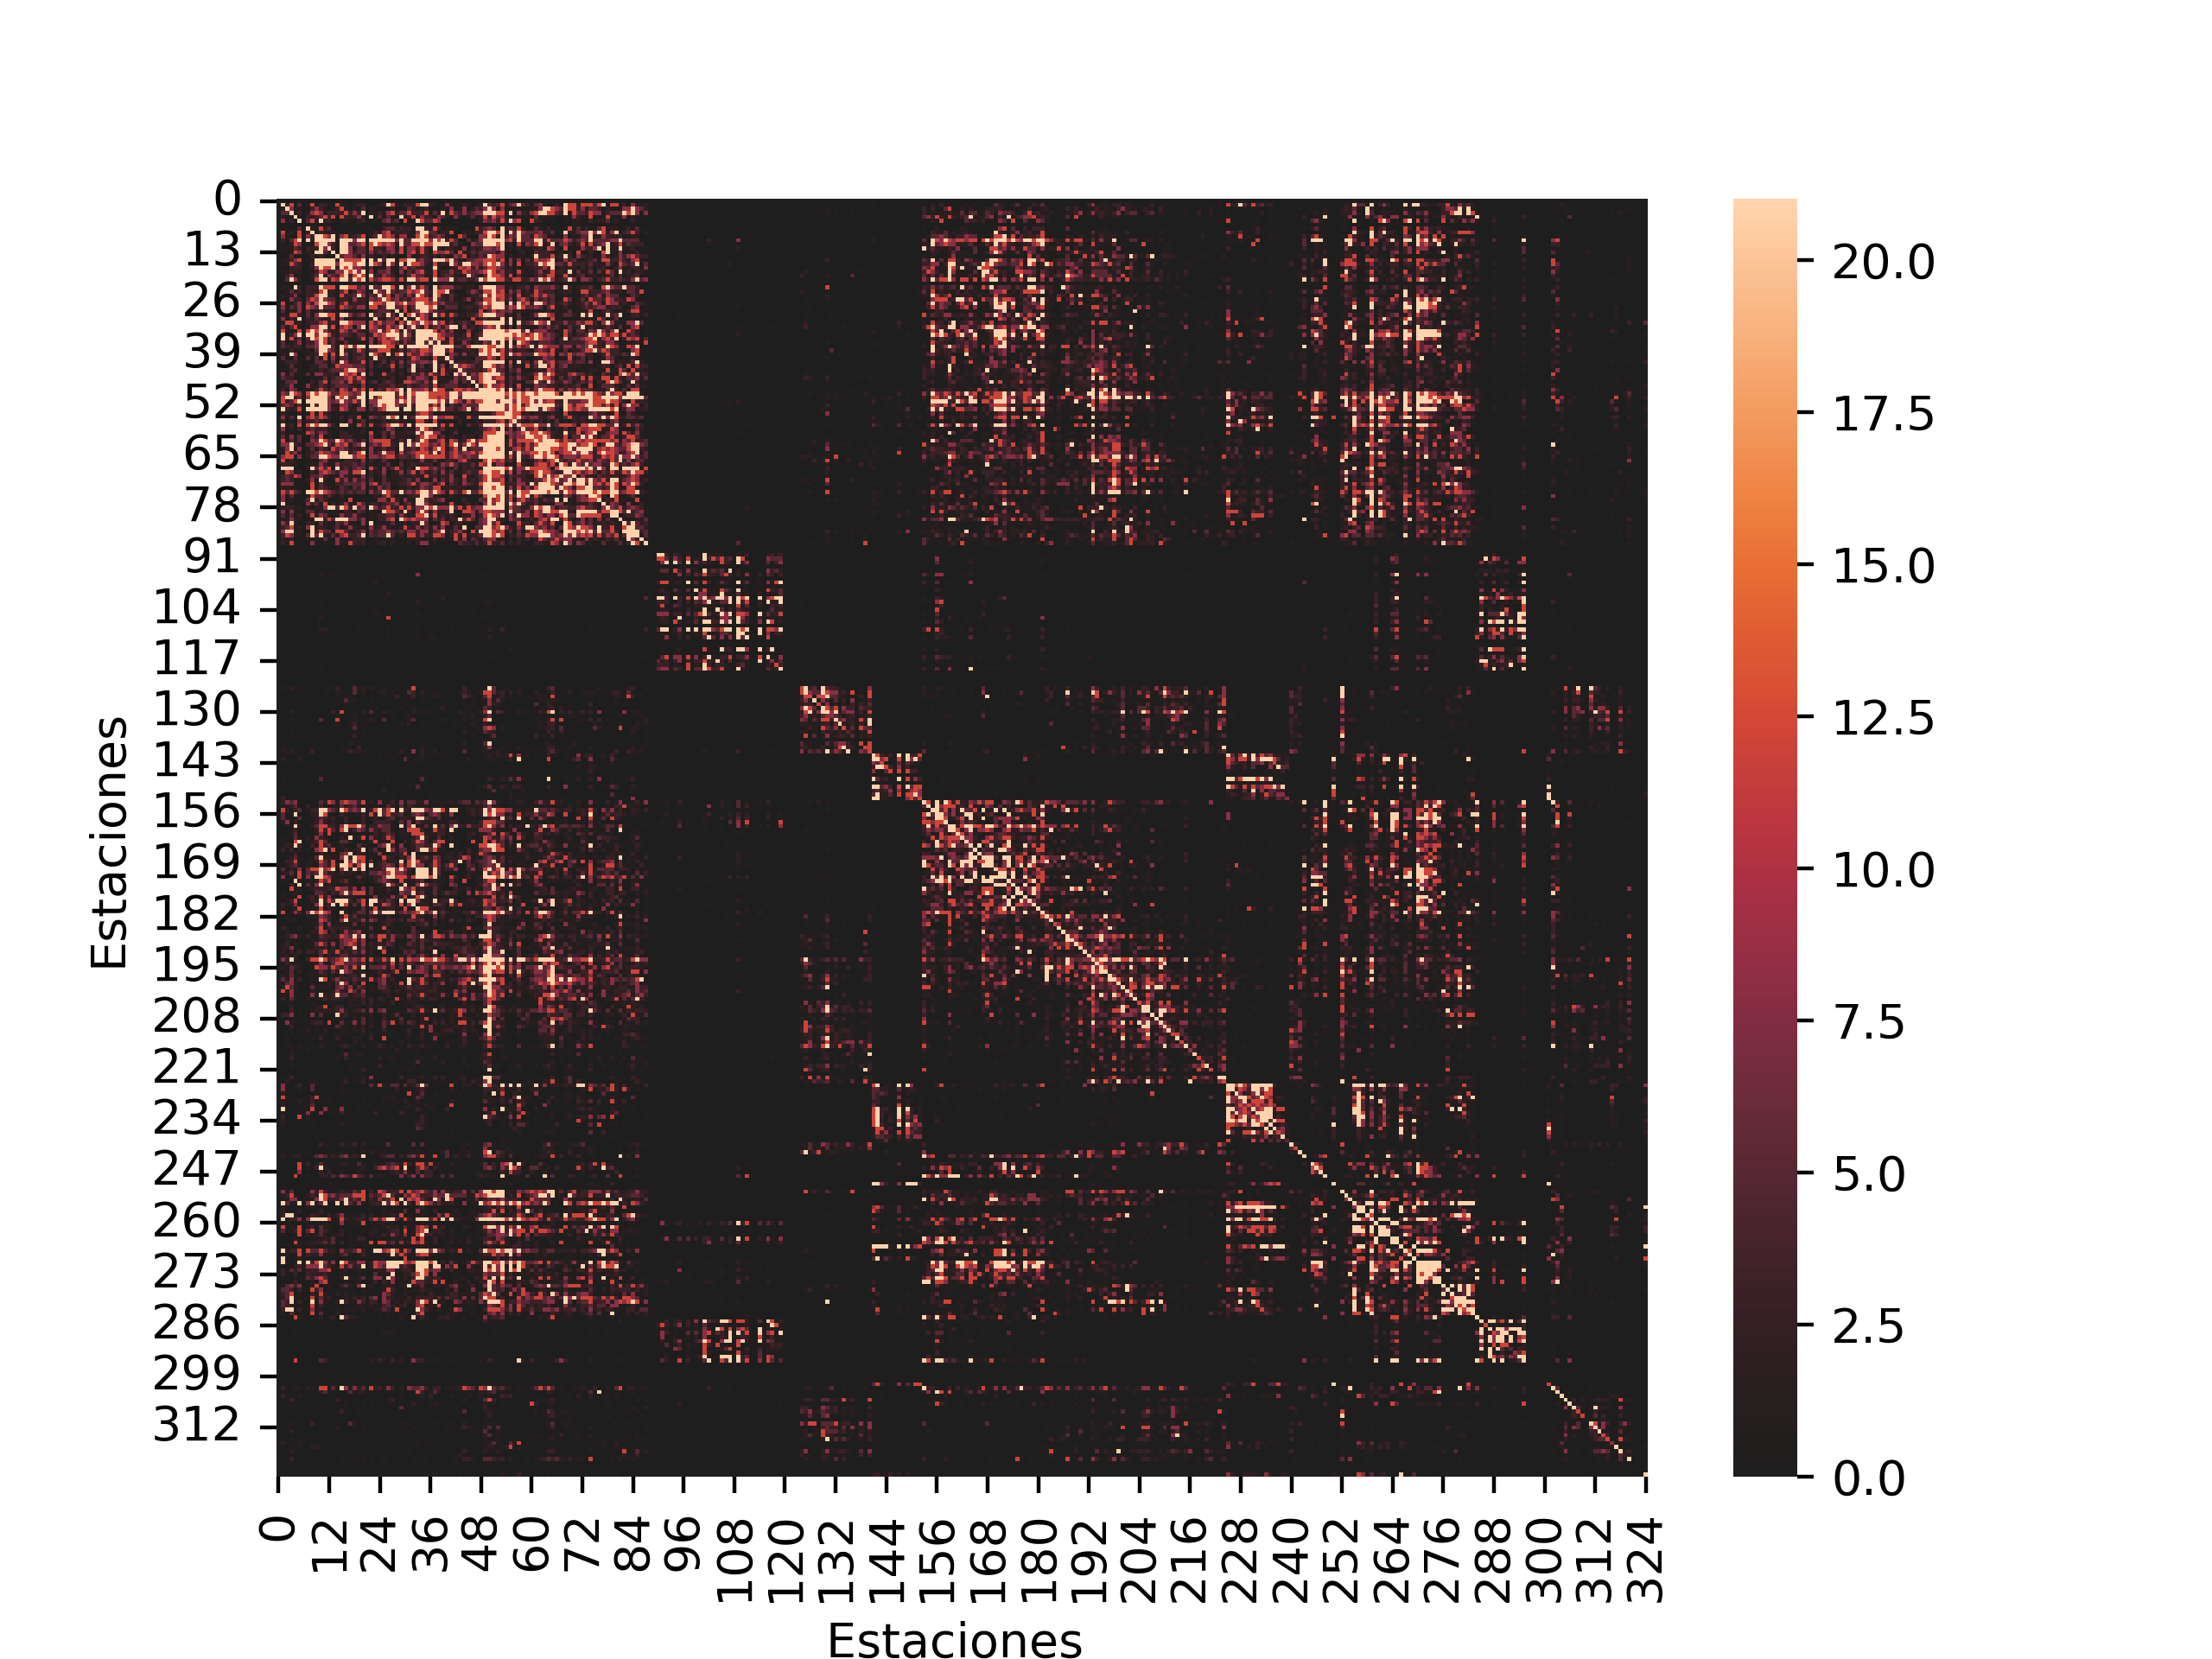
\includegraphics{/Users/jaimefco/Documents/AnalisisDeDatos/proyecto/plots/resultsSeis.png}
\caption{Etapa 6}
\end{figure}

Tomado de Mayo 2021 en adelante.

Finalente al realizarse la cuarta expansión de estaciones podemos ver
que no hay un gran cambio entre el comportamiento de las estaciones
anteriores, así como tampoco representa una gran interacción con las
estaciones establecidas anteriormente.

Hay evidencia visual para justificar los cambios en el comportamiento de
los viajes de acuerdo a los aumentos en la cantidad de estaciones, salvo
por la primera ampliación, esto puede deberse tal vez a su ubicación
geográfica pues el mapa de calor muestra que esas estaciones solo
mantienen interacción entre ellas prácticamente.

Para la realización de estos gráficos usamos una librería de
\emph{python} llamada \textbf{seaborn}, que asigna el color de acuerdo a
una escala lineal. Para evitar que los gráficos fueran muy opacos
decidimos reasigar las observaciones de acuerdo al intervalo al que
pertenecían tomando los cortes a partir de los quantiles observados e
ignorando los ceros. De esta manera, los puntos mas iluminados serán
aquellos que se encuentren por encima del 90\% de las observaciones,
siguiendo en orden descendente los que estén por encima de 80\% y así
descendentemente. Se decidió hacer de esta manera para poner más
atención a la distribución y no tanto a los máximos y mínimos.

\hypertarget{analizando-el-evento-pandemia}{%
\subsubsection{Analizando el evento
Pandemia}\label{analizando-el-evento-pandemia}}

A continuación el HeatMap del promedio de viajes promedio entre
estaciones antes del anuncio del paro a las actividades \textbf{Marzo
2020}

\begin{figure}
\centering
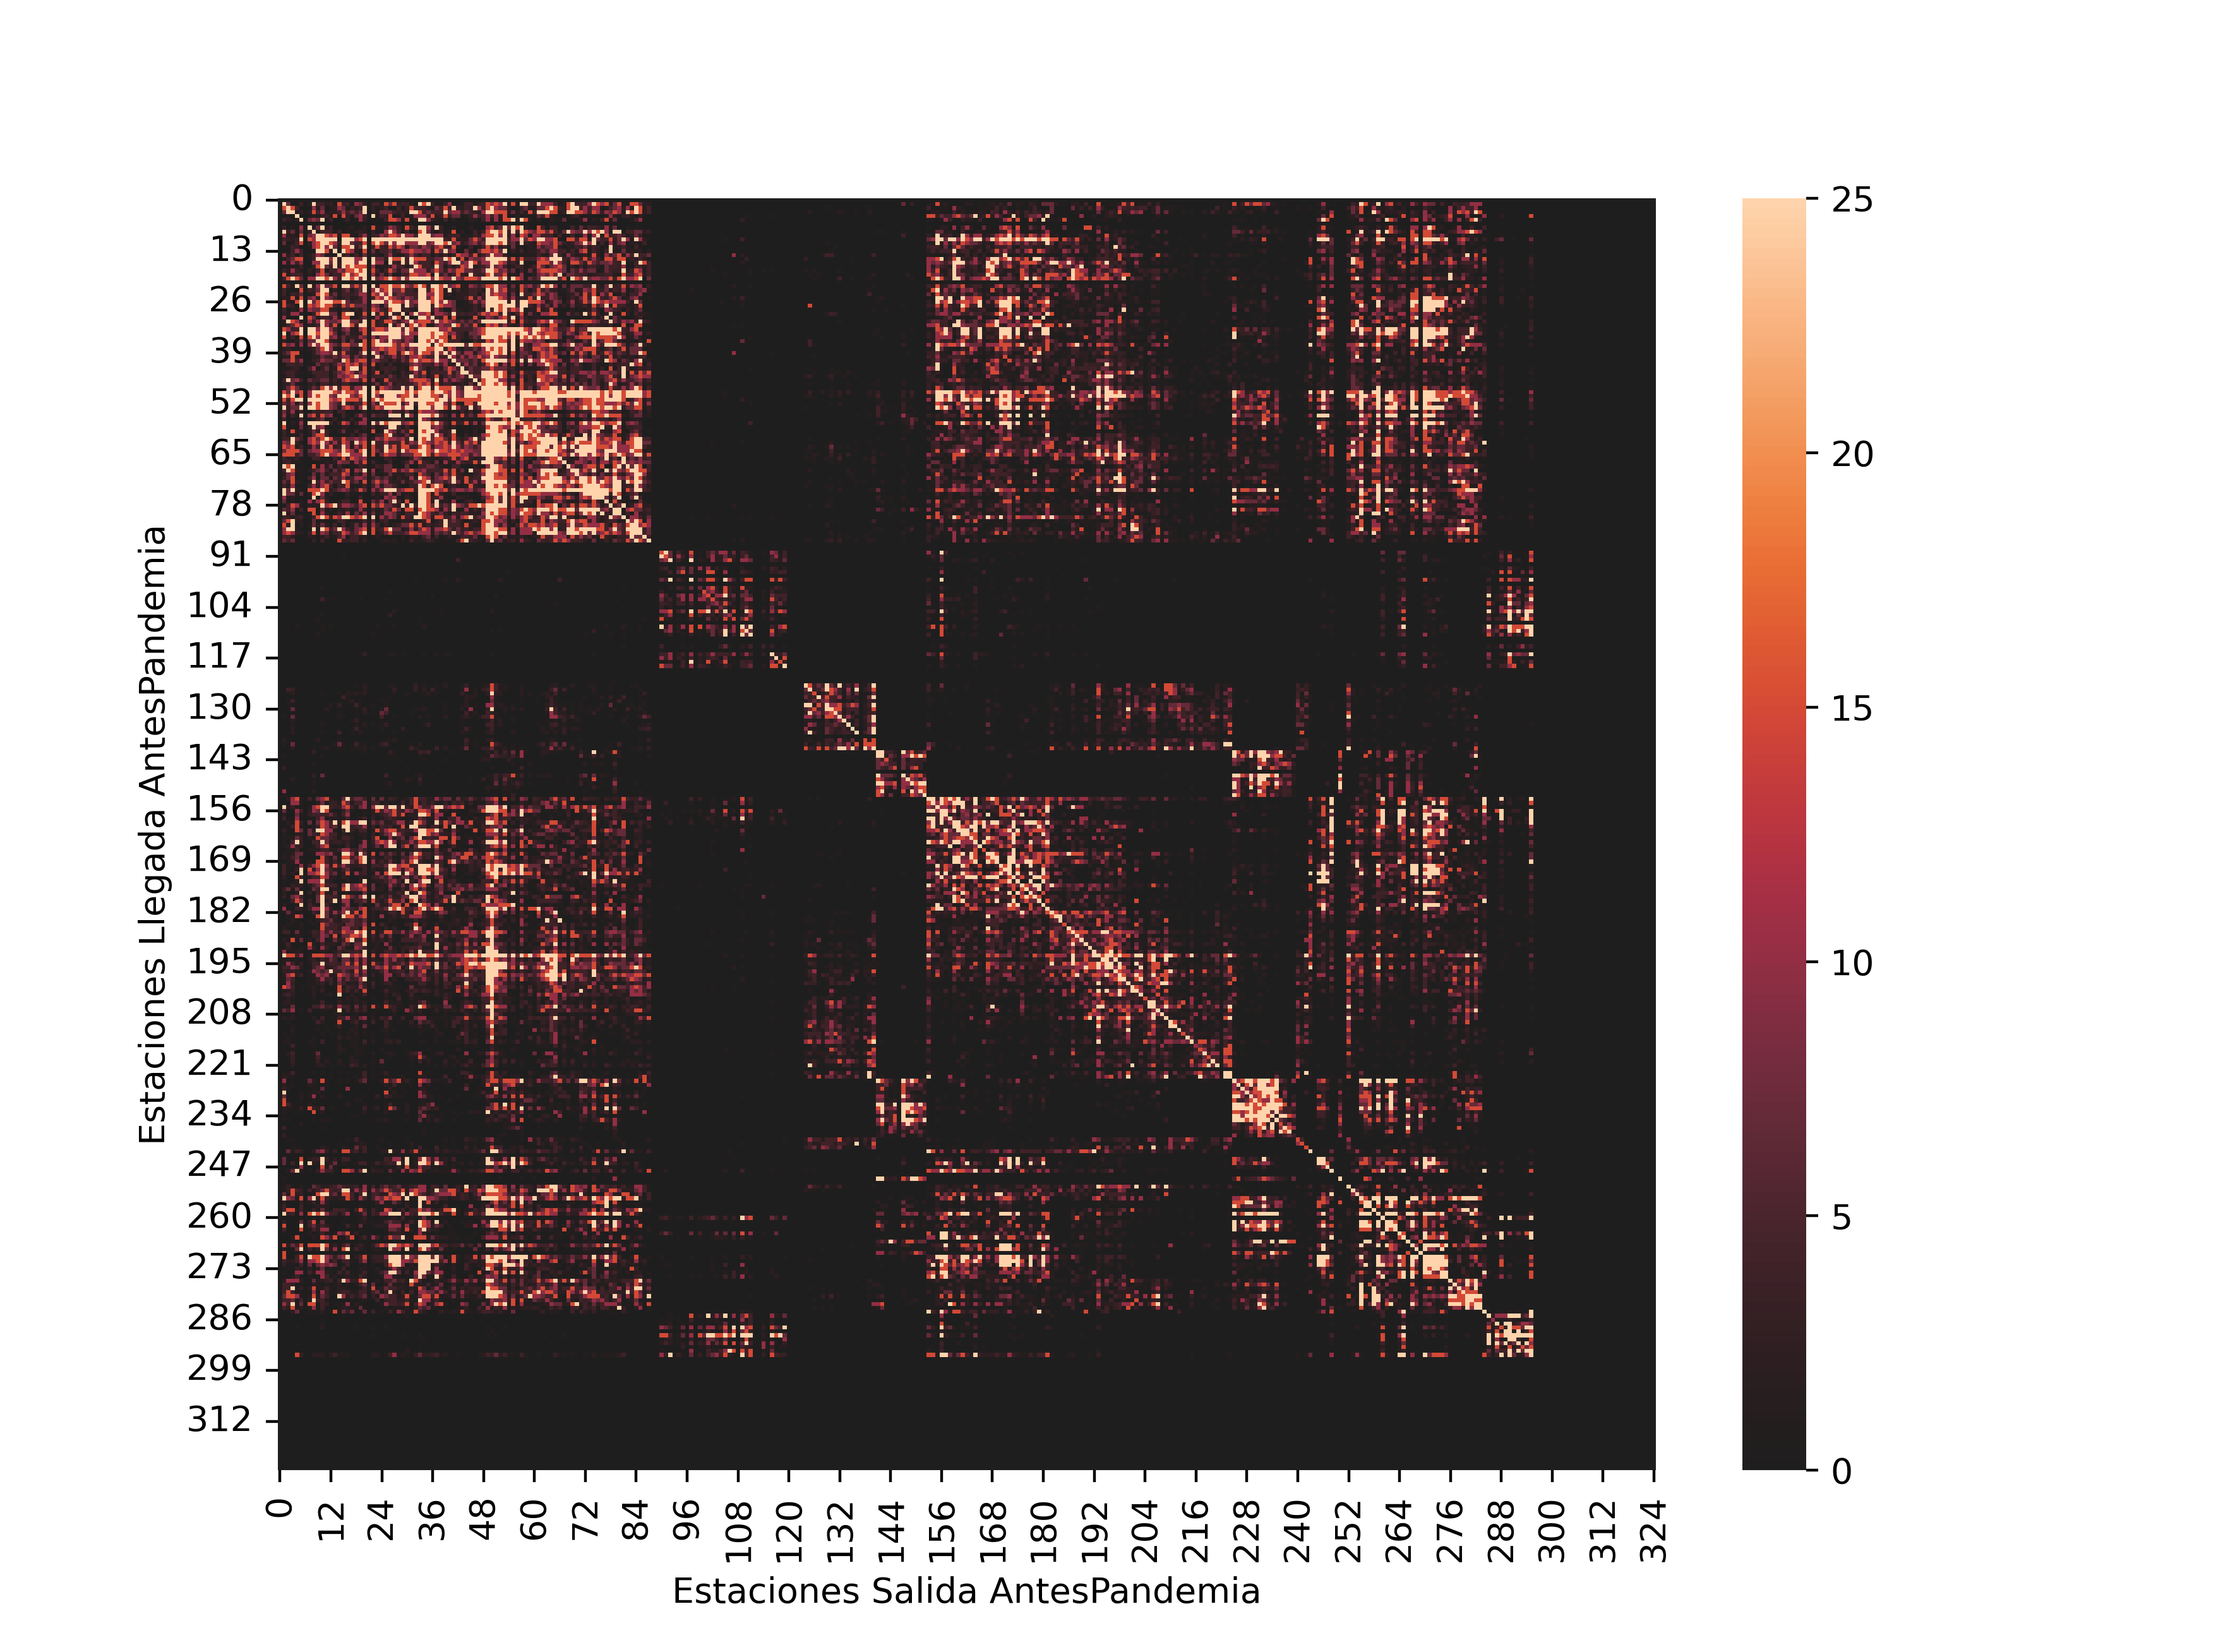
\includegraphics{/Users/jaimefco/Documents/AnalisisDeDatos/proyecto/plots/resultsAntesPandemia.png}
\caption{Antes del M1rzo 2020}
\end{figure}

Y ahora despues del llamado a quedarse en casa.

\begin{figure}
\centering
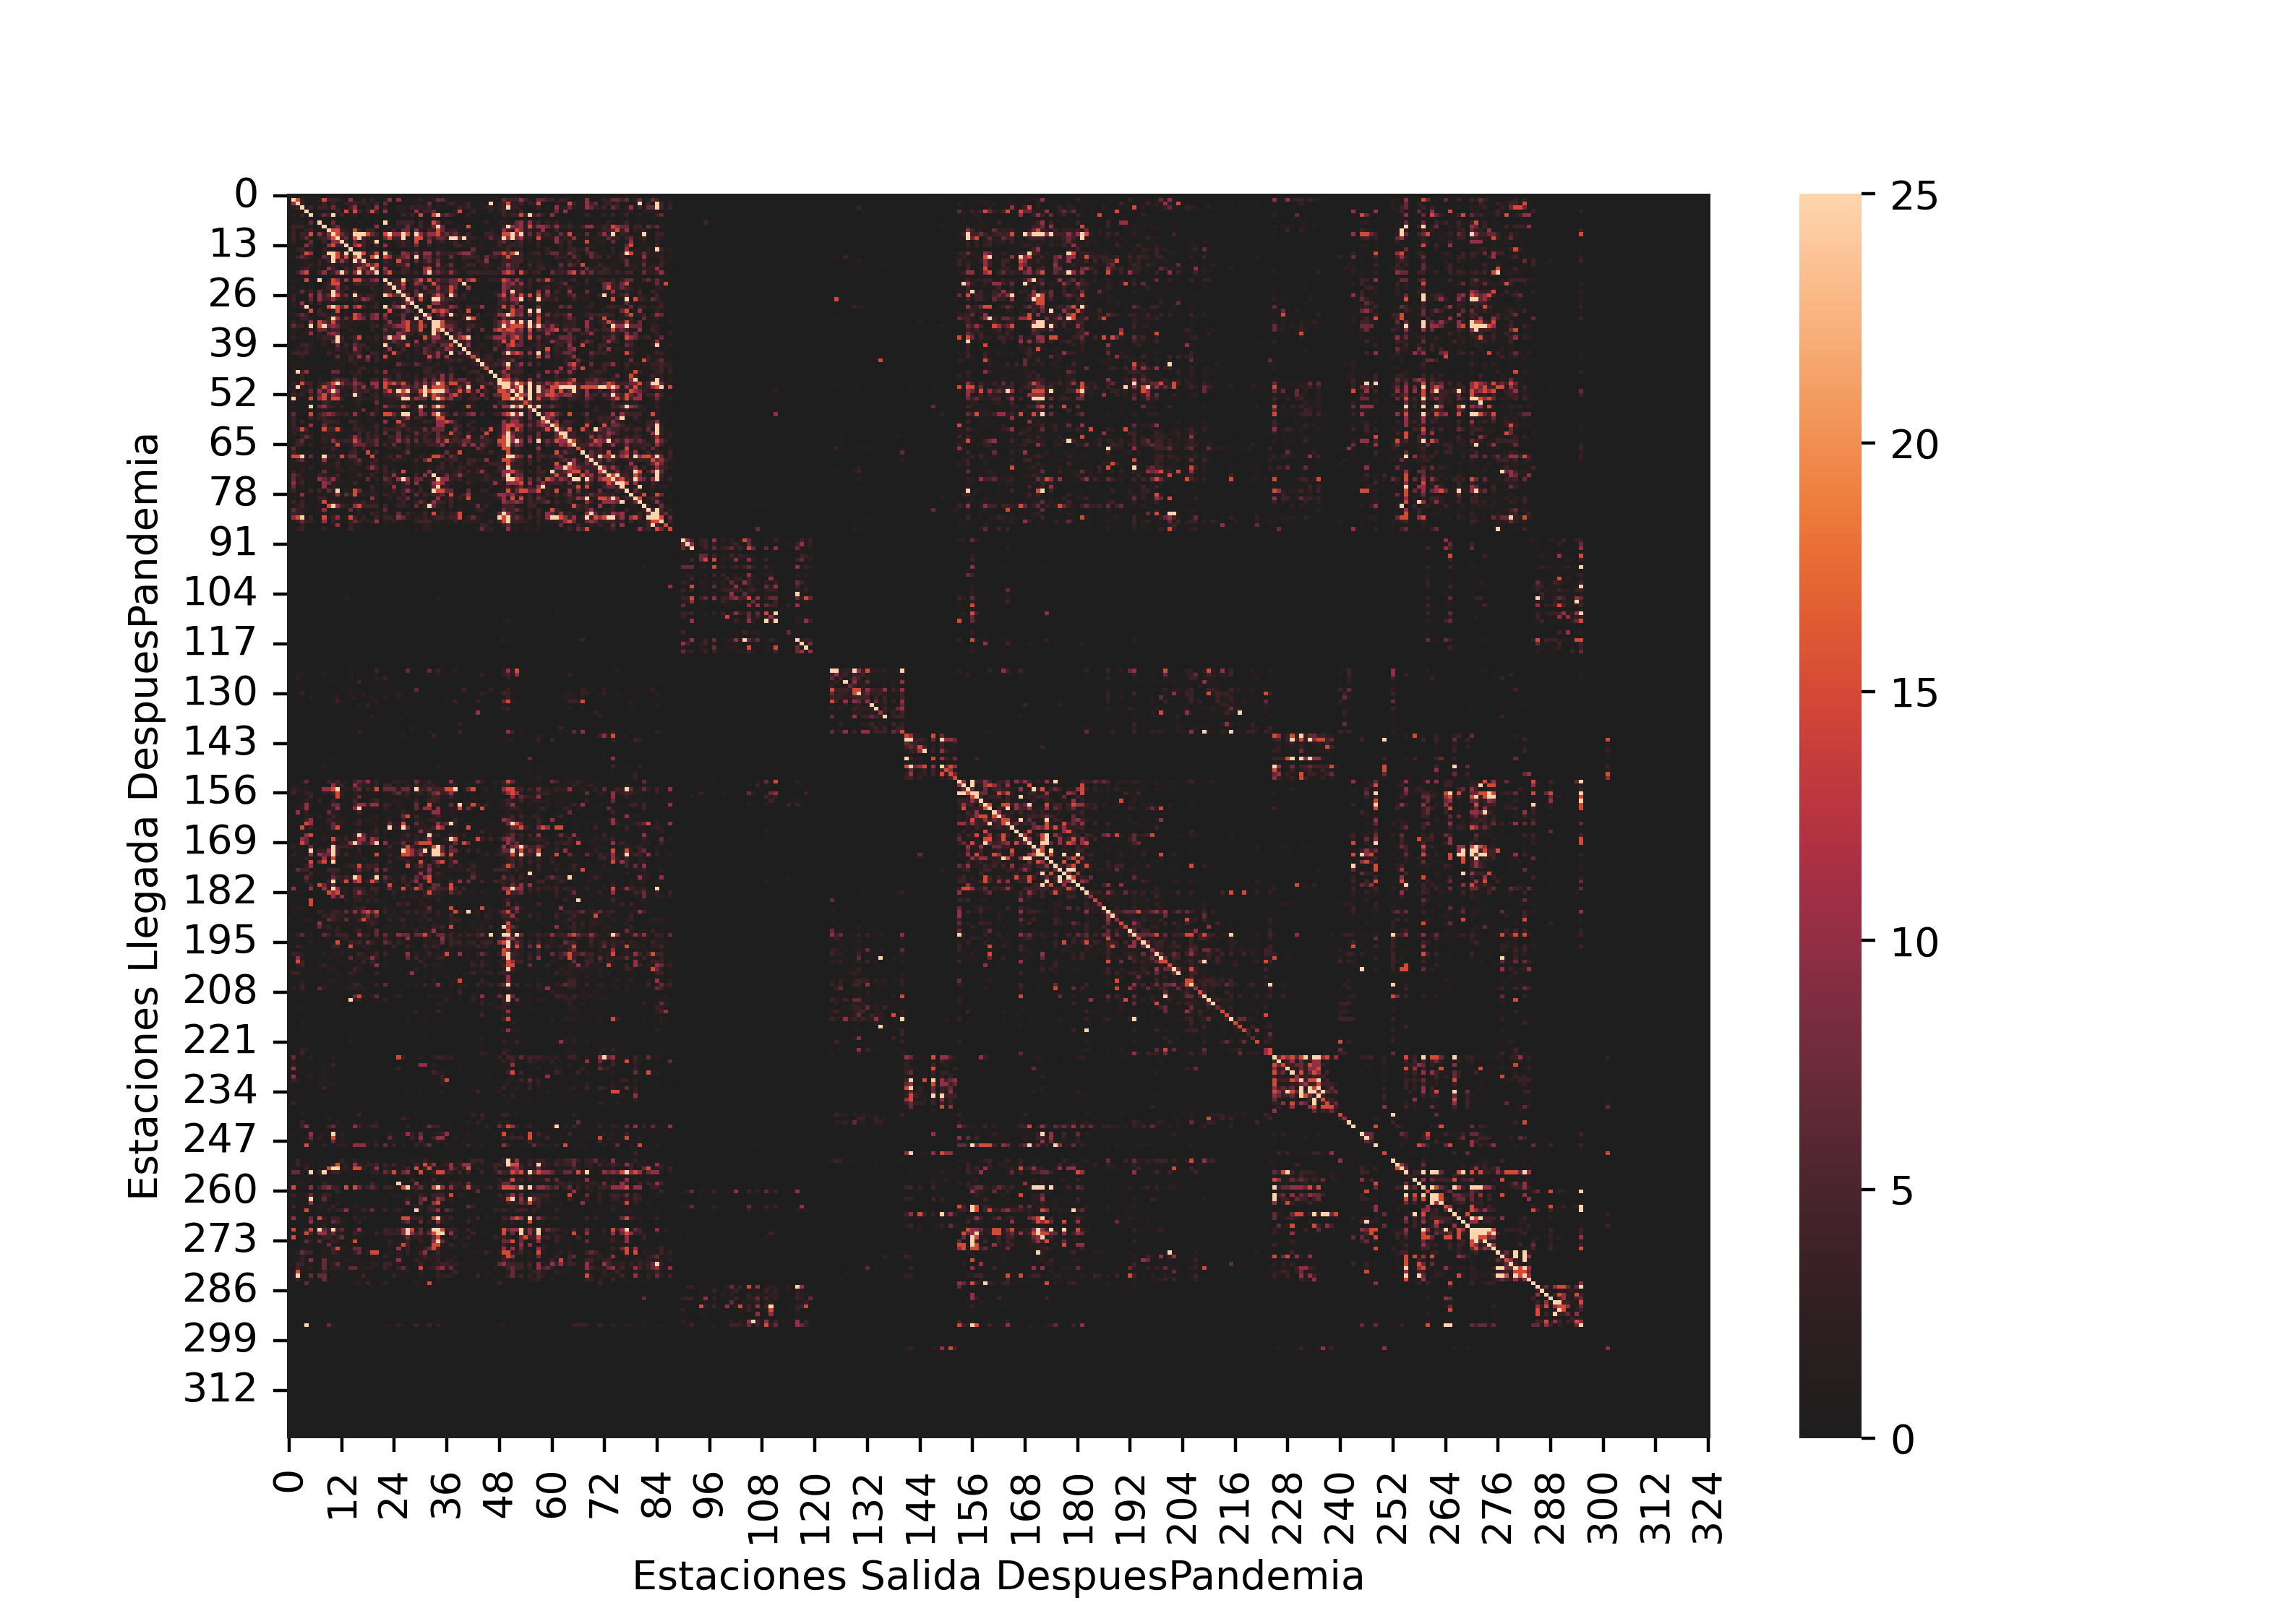
\includegraphics{/Users/jaimefco/Documents/AnalisisDeDatos/proyecto/plots/resultsDespuesPandemia.png}
\caption{Mes siguiente después de Marzo 2020}
\end{figure}

Fueron calculados en la misma escala de calor para hacer ver la
diferencia, se vuelve muy evidente la gran disminución en cuanto a
viajes.

A continuación una visualización de como se fue dando el crecimiento de
la intereacción de las estaciones.

% \begin{figure}
% \centering
% \includegraphics{/Users/jaimefco/Documents/AnalisisDeDatos/proyecto/plots/Evolucion01.gif}
% \caption{}
% \end{figure}

\begin{center}\rule{0.5\linewidth}{0.5pt}\end{center}

\hypertarget{conclusiones-y-comentarios-finales}{%
\subsection{Conclusiones y Comentarios
Finales}\label{conclusiones-y-comentarios-finales}}

\begin{itemize}
\item
  Hay evidencia significativa para afirmar que el aumentos del número de
  estaciones de las etapas 3 y 4 tuvieron un impacto positivo en el
  programa. Se destaca en particular la etapa 3. (que coinden los puntos
  de quiebre con los aumentos y se ve que las nuevas estaciones sí se
  usan y muchas de ellas conectan con las estaciones más usadas)
\item
  El impacto de las medidas de distanciamiento social es notorio en el
  uso de las bicicletas del programa (cambio de estructura más evidente,
  el heatmap...). De acuerdo al modelo de regresión lineal, se observa
  un aumento gradual de viajes.
\item
  Hay regiones fuertemente conexas, en el sentido de que la mayoría de
  viajes ocurren entre estaciones de estos conjuntos denomidos regiones.
  (estaciones muy interrelacionadas),
\item
  El impacto del aumento de estaciones fue inmediato al verse un aumento
  abruto en los viajes (explicar que es de acuerdo a lo que se observa y
  que no necesariamente refleja la realidad {[}ejemplos{]})
\item
  Un punto a tomar en cuenta es que aumentar el número de estaciones no
  garantiza un mayor uso, el mejor ejemplo de esto es que ocurrió una
  aparente ampliación en el número de estaciones en 2015 pero no
  significó una diferencia, y esto lo sustentan las observaciones
  visuales así como su no detección en los tests para puntos de quiebre.
\end{itemize}

\end{document}
